\documentclass[14pt,a4paper]{scrartcl}
\usepackage[utf8]{inputenc}
\usepackage[english, russian, ukrainian]{babel}
\usepackage{misccorr, color, ragged2e, amsfonts, amsthm, graphicx, systeme, amsmath, mdframed, lipsum, setspace, mathtools, esint, color, listings}

\renewcommand\qedsymbol{$\blacksquare$}
\renewcommand*{\proofname}{\text{Доведення}}
 \renewcommand{\labelitemi}{$\textemdash$}
\theoremstyle{definition}
\newtheorem*{defo}{Означення}
\newtheorem*{teo}{Теорема}
\newtheorem*{example}{Приклад}
\newtheorem*{remark}{Зауваження}
\theoremstyle{definition}
\newtheorem*{consequence}{Наслідок}
\theoremstyle{definition}
\newtheorem{statement}{Утверждение}[section]
\newmdtheoremenv{boxteo}{Теорема}[section]
\newtheorem*{look}{Позначення}

\setlength\parindent{0pt}

\DeclareMathOperator*\lowlim{\underline{lim}}
\DeclareMathOperator*\uplim{\overline{lim}}

\newcommand\independent{\protect\mathpalette{\protect\independenT}{\perp}}

\def\independenT#1#2{\mathrel{\rlap{$#1#2$}\mkern2mu{#1#2}}}

% Default fixed font does not support bold face
\DeclareFixedFont{\ttb}{T1}{txtt}{bx}{n}{12} % for bold
\DeclareFixedFont{\ttm}{T1}{txtt}{m}{n}{12}  % for normal

\definecolor{deepblue}{rgb}{0,0,0.5}
\definecolor{deepred}{rgb}{0.6,0,0}
\definecolor{deepgreen}{rgb}{0,0.5,0}

\doublespacing

\begin{document}

\def\be{\begin{equation}}
\def\ee{\end{equation}}

\def\bd{\begin{defo}}
\def\ed{\end{defo}}

\def\bbt{\begin{boxteo}}
\def\ebt{\end{boxteo}}

\def\i{\infty}
\def\d{\partial}

\def\vx{\overline{x}}
\def\vphi{\overline{\varphi}}
\def\vf{\overline{f}}

\begin{titlepage}
\begin{center}

\vspace*{0.1cm}
\vfill

\begin{spacing}{3}
  {\huge \textbf{ТЕОРІЯ СТІЙКОСТІ \\ ТА ВАРІАЦІЙНЕ ЧИСЛЕННЯ}}\\
\end{spacing}
\vspace{5cm}
За лекціями Горбань Н.\\
\vspace{1cm}
Редактори: Терещенко Д.\\ \hspace{3.7cm} Людомирський Ю.

\vfill

2021

\end{center}
\end{titlepage}


\tableofcontents
\newpage

\section{Лекція 1}
\subsection{Нормальні системи диференційних рівнянь}


\be
\left\lbrace
\begin{gathered}
    x'_1 (t) = f_1(t, x_1 (t), ... , x_n(t)) \\
    x'_2 (t) = f_2(t, x_1 (t), ... , x_n(t)) \\
    \vdots \\
    x'_n (t) = f_n(t, x_1 (t), ... , x_n(t)) \\
\end{gathered}\right.
\ee

 Системою диф. рівнянь n-го порядку в нормальній формі називається система вигляду (1), де $ f_i : D \to \mathbb{R}, \quad D \subset \mathbb{R}^{n+1 }, \quad i = \overline{1, n}$.
\look
\[
      \overline{x}(t) = \left[\begin{array}{l}
      x_1(t)    \\
      \dots     \\
      x_n(t)
      \end{array}\right] \text{-- невідома вектор-функція}, \quad
      \overline{f}(t, \overline{x}(t)) = \left[\begin{array}{l}
      f_1     \\
      \dots  \\
      f_n
      \end{array}\right] \text{, що}
\]
$D \rightarrow \mathbb{R}, \quad D \subset \mathbb{R}^{n+1}$, тоді $(1): \overline{x}'(t) = \overline{f}(t, \overline{x}(t))$.


\def\rect{\textbf{П}}
\bd
\textbf{Розв'язком системи} (1) на $(\alpha , \beta)$ називається така вектор-функція $\overline{x} (t) \in C^1(\alpha , \beta)$, що:
\begin{enumerate}
  \item $(t, x_1(t), \dots, x_n(t)) \in D \quad \forall t \in (\alpha, \beta)$;
  \item $\overline{x}(t)$  перетворює $(1)$ на тотожність на інтервалі $(\alpha, \beta)$.
\end{enumerate}

\textbf{Загальним розв'язком системи}  (1) називається n-параметрична сім'я розв'язків (1), що охоплює всі розв'язки системи.
\ed

Задача Коші. Для заданих $t_0, \overline{x}^{0} \in D$ знайти такий розв'язок (1), що $\overline{x} (t_0) = \overline{x}^{0}$.
Нехай $\Pi = \{(t, \overline{x}) \in \mathbb{R} \quad \big| \quad |t-t_0| \leq a, \quad ||\overline{x} - \overline{x}_0|| \leq b \}$.

\begin{boxteo}[Теорема Пеано]
Нехай $\overline{f} \in C(\Pi)$. Тоді розв'язок задачі Коші:
\begin{gather*}
  \begin{cases}
    \overline{x}' = \overline{f}(t, \overline{x}) \\
    \overline{x}(t_0) = \overline{x}_0
  \end{cases}
\end{gather*}
існує принаймні на проміжку $I_h = (t_0 - h, t_0 + h)$, де $h = \min\{{a, \dfrac{b}{M}}\}$, \\ $M = \max\limits_{(t, x) \in \Pi} {||\overline{f}(t, \overline{x})||}$.
\end{boxteo}

\begin{boxteo}[про продовження]
Нехай для системи (1) виконується, що $\overline{f} \in C(D), \quad D \subset \mathbb{R}^{n + 1}$ -- обмежена область. Тоді $\forall t : (t_0, \overline{x}_0) \in D$ існують такі $t^{-}, t^{+} : t^{-} < t_0 < t^{+}$, що розв'язок системи (1) з початкової умови $\overline{x}(t_0) = \overline{x}_0$ існує на інтервалі $(t^{-}, t^{+})$, причому $(t^{-}, \overline{x}(t^{-})) \text{ та } (t^{+}, \overline{x}(t^{+}))$ належать межі області $D$.
    \begin{center} 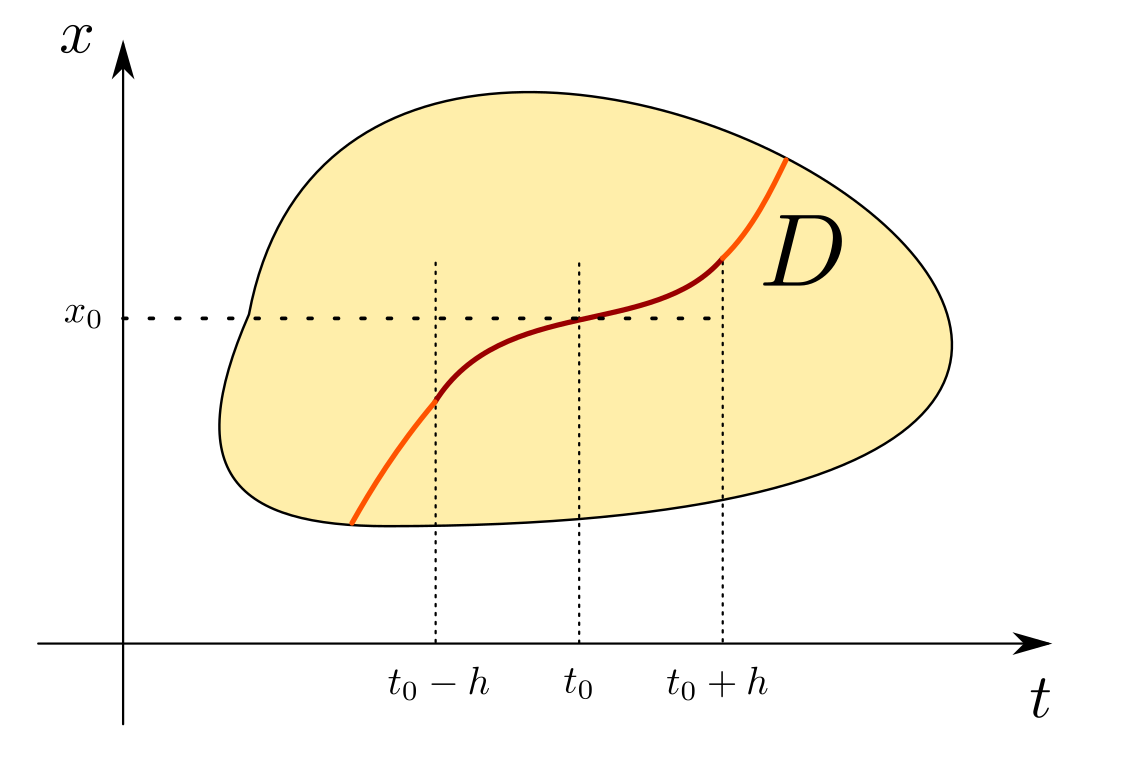
\includegraphics[scale=0.35]{assets/lect0.png} \end{center}
\end{boxteo}

\begin{boxteo}[Теорема Пікара]
  Нехай
  \begin{spacing}{1}
  \begin{enumerate}
    \item $\overline{f} \in C(\Pi)$;
    \item $\exists! L > 0 : \forall (t_1, \overline{x}_1), (t_2, \overline{x}_2) \in \Pi$ справедливо, що $|| f(t_1, \overline{x}_1) - f(t_2, \overline{x}_2)|| \leq \\ \leq L||\overline{x}_1 - \overline{x}_2||$ (умова Ліпшиця).
  \end{enumerate}
  \end{spacing}


  Тоді $\exists!$ розв'язок задачі Коші з початкової умови $\overline{x}(t_0) = \overline{x}_0(t)$, визначений принаймні на $I_h = (t_0 - h, t_0 + h), \quad h = \min\{{a, \dfrac{b}{M}}\}, \quad M = \max\limits_{\Pi}||f(t, \overline{x})||$.
\end{boxteo}

\subsection{Основні поняття теорії стійкості.}
Розглянемо систему диференційних рівнянь $\overline{x}' = \overline{f}(t, \overline{x})$ (1), де $f : D \rightarrow \mathbb{R}^n$ та $D = [a, +\infty) \times G, \quad G \subset \mathbb{R}^n$. Нехай при цьому $\overline{f}$ задавольняє умовам існування та єдиності розв'язку задачі Коші в будь-якій точці $(t_0, \overline{x}_0) \in D$

\bd
Розв'язок $\overline{x} = \overline{\varphi}(t)$ системи (1) називається \textbf{стійким} за Ляпуновим, якщо

\begin{enumerate}
  \item $\overline{x} = \overline{\varphi}(t) \quad \exists  \text{ на } [a, +\infty)$ (відсутніть вертикальних асимптот)
  \item $\forall \varepsilon > 0 \quad \forall t_0 \geq a \quad \exists \delta > 0 : \forall $ розв'язку $\overline{x}(t)$ системи (1) такого, що $||\overline{x}(t_0) - \overline{\varphi}(t_0)|| < \delta$ виконується наступне, що $\overline{x}(t)$ існує на $[t_0, +\infty)$ та $||\overline{x}(t) - \overline{\varphi}(t)|| < \varepsilon \quad \forall t \geq t_0$.
\end{enumerate}
\ed

\begin{center} 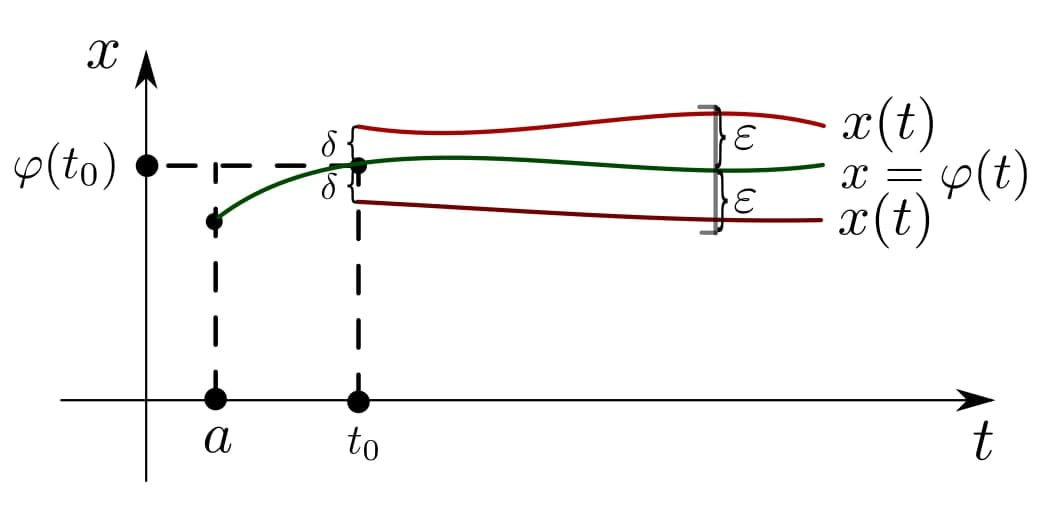
\includegraphics[scale=0.35]{assets/lect1.jpg} \end{center}

\bd
Розв'язок $\overline{x} = \overline{\varphi}(t)$ системи (1) називається \textbf{асимптотично стійким} за Ляпуновим, якщо

\begin{enumerate}
  \item $\overline{x} = \overline{\varphi}(t)$ стійкий;
  \item $\forall t_0 \geq a \quad \exists \delta > 0: \forall$ розв'язку $\overline{x}(t)$ с-ми (1) такого, що $||\overline{x}(t_0) - \overline{\varphi}(t_0)|| < \delta$ справедливо, що $||\overline{x}(t_0) - \overline{\varphi}(t_0)|| \rightarrow 0 \text{ при } t \rightarrow + \infty$.
\end{enumerate}

\begin{center} 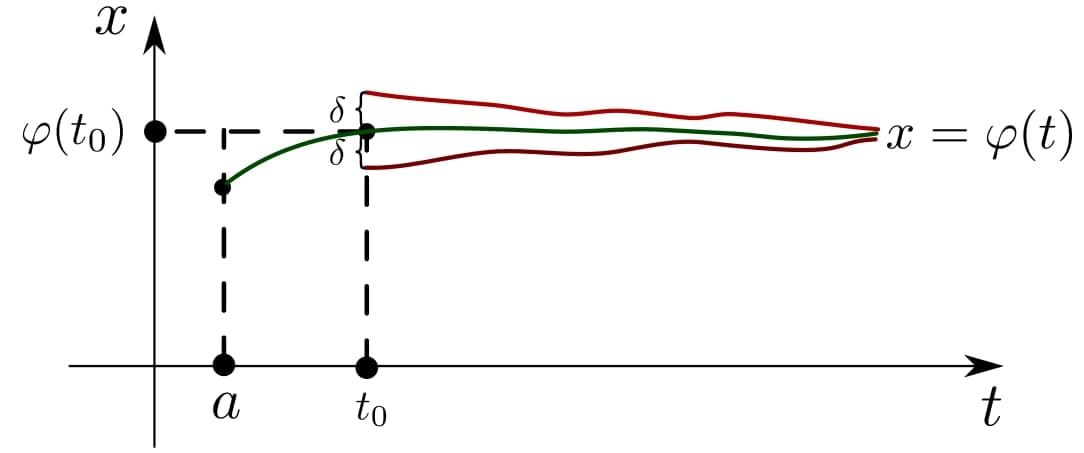
\includegraphics[scale=0.35]{assets/lect2.jpg} \end{center}

Роз'язок $\overline{\varphi}(t)$ називається \textbf{нестійким за Ляпуновим}, якщо він не є стійким, тобто:
\ed

\begin{enumerate}
  \item Або $\overline{x} = \overline{\varphi}(t) \quad \nexists$ на  $[a, +\infty)$ (вертикальні асимптоти);
  \item Або $\exists \varepsilon > 0 : \exists t_0 \geq a :  \forall \delta > 0$ існує розв'язок $\overline{x}(t)$ системи (1) такий, що $||\overline{x}(t_0) - \overline{\varphi}(t_0)|| < \delta$, але $||\overline{x}(t_0) - \overline{\varphi}(t_0)|| > \varepsilon$
\end{enumerate}

\vfill
\begin{center} 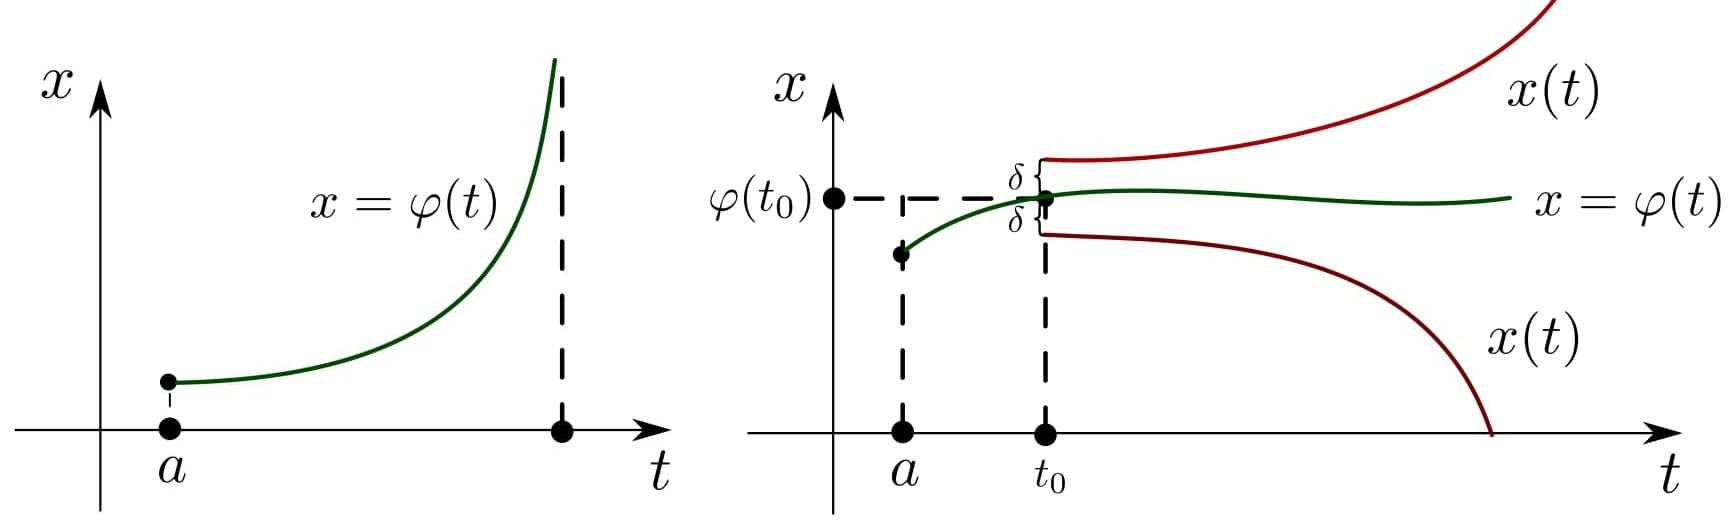
\includegraphics[scale=1.15]{assets/lect3+4.jpg} \end{center}
\vfill
\subsection{Приклади дослідження на стійкість за означенням.}

\begin{example}
    Дослідити на стійкість розв'язок задачі Коші:
$$
\begin{cases}
    x' = 1 \\
    x(0) = 0
\end{cases}
$$

\begin{enumerate}
\item Знайдемо розв'язок заданої задачі Коші: $x = 1 \Rightarrow x = t + C$ - загальний розв'язок. Підставимо: $ x(0) = 0 \quad \Rightarrow \quad 0 = 0 + C \quad \Rightarrow \quad C = 0 \quad \Rightarrow \quad$ \fbox{ $ \varphi(t) = t $} -- розв'язок, який будемо досліджувати.
Зазначений розв'язок не має вертикальних асимптот та $\exists$ на $\mathbb{R}$.

\item Знайдемо розв'язок довільної задачі Коші $x(t_0) = x_0$.
$$
x_0 = t_0 + C \quad \Rightarrow \quad C = x_0 - t_0 \quad \Rightarrow \quad x(t) = t + x_0 - t_0
$$
\item Нехай $  \left| x(t_0) - \varphi(t_0) \right|  =  \left| x_0 - t_0 \right| < \delta$, тоді $ \left| x (t) - \varphi (t) \right|  = \left|  x_0 - t_0 \right| < \varepsilon = \delta $.\\
Таким чином, розв'язок є стійким, але не є асимптотично стійким.

\end{enumerate}

\end{example}

\begin{example}
    Дослідити на стійкість розв'язок  задачі Коші:
    $$
    \begin{cases}
        x' = 1 + t - x \text{  -- лінійне неоднорідне рівняння першого порядку}\\
        x(0) = 0
    \end{cases}
    $$
    \begin{enumerate}

    \item Знайдемо розв'язок даної задачі Коші:
    $$
    x' = - x + 1 + t = \left| \text{ метод Бернуллі, } x = uv \right| = t + Ae^{-t}
    $$
    Знайшли загальний розв'язок. Із умови задачі Коші: $ A = 0 \Rightarrow \fbox {$\varphi(t) = t$ }$

    \item Знайдемо розв'язок довільної задачі Коші:
    $$
    x(t_0) = x_0, \quad x_0 = t_0 + Ae^{-t_0} \quad \Rightarrow \quad A = (x_0 - t_0) e^{t_0}
    $$
    Отримали: $x(t) = t + (x_0 - t_0) e^{t_0 - t} - \text{ загальний розв'язок задачі Коші}$

    \item Беремо $\left| x(t_0) - \varphi(t_0) \right| = |t_0 - x_0| < \delta$ і розглянемо:
    $$\left| x(t) - \varphi(t) \right| = |t - t - (x_0 - t_0)e^{t_0 - t}| < \delta e^{t_0 - t} \rightarrow 0, \text{ при } t \rightarrow + \infty$$
    Отже, $\forall t_0 \quad \exists \delta > 0 :$ для будь-якого розв'язку $x(t): |x(t_0) - \varphi(t_0)| = |x_0 - t_0| < \delta$ справедливо, що $|x(t) - \varphi(t)| \rightarrow 0 \text{ при } t \rightarrow + \infty$. Отримали, що розв'язок даної задачі Коші $\varphi(t) = t$ є асимптотично стійким.
    \end{enumerate}
\end{example}

\remark
Очевидно, що простіше досліджувати на стійкість розв'язок типу $\varphi(t) = 0$. Нехай (1) $\overline{x}'(t) = \overline{f}(t, \overline{x})$, а $\overline{x} = \overline{\varphi(t)}$ -- розв'язок, який потрібно дослідити на стійкість. Застосуємо заміну: $\overline{z} = \overline{x} - \overline{\varphi}(t), \text{ де } \overline{z}$ -- нова невідома вектор-функція. Отримаємо систему:
$$
\overline{z}'(t) + \overline{\varphi}'(t) = \overline{f}(t, \overline{z} + \overline{\varphi}(t)) \quad \Rightarrow \quad \overline{z}'(t) = \overline{f}(t, \overline{z} + \overline{\varphi}(t)) - \overline{f}(t, \overline{\varphi}(t)) \quad (*)
$$
Можно довести, що розв'язок $\overline{x} = \overline{\varphi}(t)$ системи (1) -- стійкий (асимптотично стійкий або нестійкий) $\Longleftrightarrow$ розв'язок $\overline{z} = \overline{0}$  cистеми $(*)$ -- стійкий (асимптотично стійкий або нестійкий).

\subsection{Стійкість розв'язків лінійних систем}
Лінійна неоднорідна система рівнянь n-ого порядку має вигляд (далі ЛНС):
\be
\overline{x}' = A(t) \overline{x} + \overline{f} (t).
\ee

$ \text{Де } A(t) \in \mathbb{R}^{n \times n}, \quad A(t) \in C [ a, + \infty), \quad \overline{f} \in C[a, + \infty)$ \\

Тоді $\forall t_0 \geq a, \quad \forall \overline{x}_0 \in \mathbb{R}^n \quad$ існує єдиний розв'язок ЛНС (2) з початковими умовми $\overline{x}(t_0) = \overline{x}_0$, визначений на $[a, +\infty)$.

Нехай $\overline{\varphi}(t)$ -- розв'язок (2), який потрібно дослідити на стійкість.
Застосуємо заміну: $ \overline{z} (t) = \overline{x} - \vphi (t)$, де $ \overline{z}(t)$ - нова невідома вектор-функція, а $\vphi (t)$ - розв'язок, який ми маємо дослідити на стійкість.

Отримали лінійну однорідну систему першого порядку (далі ЛОС):

$$ \overline{z}'(t)   + \vphi'(t) = A(t)\overline{z}(t) + A(t)\vphi(t) + \overline{f}(t) $$
\be
\overline{z}' = A(t) \overline{z} \text{ -- ЛОС n-ого порядку}
\ee

Заміною ми звели дослідження довільного розв'язку лінійної неоднорідної системи до дослідження нульового розв'язку відповідної ЛОС. Таким чином, приходимо до висновку, що усі розв'язки є одночасно стійкими, асимптотично стійкими або не стійкими. А отже, розглядаючи будь-яку лінійну систему, можемо говорити про стійкість не окремого розв'язку, а системи в цілому. Досліджуючи при цьому розв'язок $\overline{x}(t) = \overline{0}$\\

Розв'яжемо ЛОС (3) (перейдемо до змінної $x$): $\quad \overline{x}'  =  A(t) \overline{x} $ -- ЛОС (3).

$X(t) $ -- її фундаментальна матриця (далі позначаємо ФМ). Тоді загальний розв'язок: $ \overline{x} (t) = X(t) \cdot \overline{C}$, де $\overline{ C} \in \mathbb{R}^n$.
Розв'язок задачі Коші з початковими умовами $ \overline{x} (t_0) = \overline{x_0}$:
$$
\overline{x}_0 = X(t_0) \cdot \overline{C} \Rightarrow \overline{C} = X^{-1} (t_0) \cdot \overline{x_0} \Rightarrow \fbox{$x(t) = X(t) X^{-1}(t_0) \overline{x}_0$}
$$

\begin{spacing}{2.5}
  \begin{boxteo}[Про стійкість ЛОС]\quad \\
  а) (3) - стійка $\Longleftrightarrow \exists K > 0: \sup\limits_{t\geq  a} ||X(t) || \leq K$.\\
  б) (3) - асимптотично стійка $\Longleftrightarrow  ||X(t)|| \to 0 $, при $ t \to +\infty$.\\
  в) (3) - нестійка. $ \Longleftrightarrow \exists \left\lbrace t_n \right\rbrace_{n=1}^{\infty} : ||X(t_n)|| \to +\infty $, при $n \to \infty$
  \end{boxteo}
\end{spacing}

\begin{spacing}{2.25}
\textbf{Доведення.} а) \fbox{$\Longleftarrow$} \\ Нехай $ \exists K > 0 : \sup\limits_{t\geq a} ||X(t)|| \leq K$.

 Доведемо стійкість розв'язку $\overline{x} (t) = \overline{0}.$ За означенням, візьмемо розв'язок довільної задачі Коші з початковими умовами $\overline{x } (t_0) = \overline{x}_0$.
Нехай $|| \overline{x}_0 || < \delta$ і розглянемо $ || \overline{x} (t)|| = || X(t) \cdot X^{-1} (t_0) \cdot \overline{x}_0 || \leq ||X(t)|| \cdot || X^{-1} (t_0)|| \cdot || \overline{x}_0|| \leq K \cdot || X^{-1} (t_0)|| \cdot || \overline{x}_0|| < K || X^{-1} (t_0)||\delta < \varepsilon $ при $ \delta = \dfrac{\varepsilon }{K || X^{-1} (t_0)|| + 1} $.
Отже, $\forall t_0 \geq  a \quad \forall \varepsilon >0 \quad \exists \delta > 0 \quad \left(  \delta = \dfrac{\varepsilon }{K || X^{-1} (t_0)|| + 1}  \right)$  для довільного розв'язку з $ || \overline{x}_0|| < \delta$ справедливо $ ||\overline{x} (t)|| < \varepsilon  \quad \Longrightarrow \quad $ стійкість розв'язку. $\blacksquare$  \\
\end{spacing}
\textbf{Доведення.} a) \fbox{$\Longrightarrow$} \\ Нехай (3) -- стійка. Припустимо від супротивного, що

$$\exists  \left\lbrace t_n \right\rbrace_{n\geq 1}^{\infty} : t_n \rightarrow +\infty : ||X(t_n)|| \to {+\infty} \text{ при } n \to \infty$$\\
Тоді $\exists j = \overline{1, n} : || \overline{x}^{j} (t_n)|| \to \infty$, де $\overline{x}^j$  - це $j$-тий стовпчик ФМ. \\ Покладемо $\forall \delta > 0:$


$$
\overline{x}^{\delta}_0 = \frac{\delta X(t_0) \overline{e}_j}{2 ||X(t_0)||} \text{ , де }\overline{e}_j = \begin{bmatrix}
 0\\
 \vdots\\
 1\\
 \vdots\\
 0
\end{bmatrix} - j
$$

Тоді $|| \overline{x}_0^{\delta}|| = \dfrac{1}{ 2 ||X(t_0)||}  \cdot \delta ||X(t_0) \cdot \overline{e}_j|| < \delta $.\\
Розглядаємо розв'язок задачі Коші з початковими умовами $ \overline{x} (t_0) = \overline{x} _0 ^ \delta$. Маємо:
$$
\overline{x} (t) = X(t) \cdot X^{-1}(t_0) \cdot \overline{x}_0 ^\delta = X(t) X^{-1} (t_0) \cdot \dfrac{ \delta X(t_0) \overline{e}_j}{ 2 ||X(t_0)||} = \frac{\delta}{2} \cdot \frac{X(t) \overline{e}_j}{ ||X(t_0)||} = \frac{\delta}{2 ||X(t_0)|| } \cdot \overline{x}^j (t)
$$
$$
\Longrightarrow \forall \varepsilon >0 \quad \exists n_0 \in \mathbb{N} \quad : \forall n \geq n_0
$$
$$
||\overline{x} (t_n)|| = \frac{\delta}{ 2 ||X(t_0)|| } \cdot ||\overline{x}^j (t_n)|| \to \infty > \varepsilon
$$
Отримали нестійкість системи $ \Rightarrow  $ суперечність початковій побудові $ \Rightarrow$ a).\\
Пункт б) доводиться аналогічно а). $\quad$ Пункт в) випливає із пукнта а). $\quad \blacksquare$

\subsection{Стійкість ЛОС зі сталою матрицею.}

\begin{equation}
\overline{x} ' (t) = A \overline{x} (t) \text{, де $A$ - стала матриця $n \times n$}
\end{equation}
\begin{boxteo} \quad \\
a) (4) - стійка $ \Longleftrightarrow  \forall \lambda $ - власне число матриці $A$: \\
$\Re \lambda \leq 0$, причому якщо $ \Re \lambda = 0$, то йому відповідають лише одновимірні клітини Жордана. \\
б) (4) - асимптотично стійка $ \Longleftrightarrow \forall \lambda $ - власні числа матриці $A: \Re \lambda < 0 $.\\
в) (4) - нестійка $ \Longleftrightarrow $ не є стійкою.
\end{boxteo}

\textbf{Доведення.} Нехай $ \lambda = \alpha + i\beta$ - власне число матриці $A \Rightarrow $ у ФМ цьому власному числу відповідає розв'язок: \\
  - якщо $ \lambda$ відповідають лише одновимірні клітини Жордана:
  $$
  \overline{x} (t) = e^{\alpha t} ( \overline{Q} _0 \cos{(\beta t)} + \overline{R}_0 \sin{(\beta t)} )
 $$
 - якщо клітина Жордана розміру $l$:
 $$
 \overline{x} (t) = e^{\alpha t} ( \overline{Q} _{l-1} \cos{(\beta t)} + \overline{R}_{l-1} \sin{(\beta t)} )
 $$
 Тоді:\\
якщо $ \Re \lambda = \alpha < 0  \Rightarrow || \overline{x} (t)|| \to 0 $ за $t \to \infty$.\\
якщо $ \Re \lambda = \alpha >0 \Rightarrow || \overline{x} (t)|| \to + \infty $ за $t \to \infty$.\\
якщо $ \Re \lambda = 0 $, то:\\
\hspace*{1cm} - якщо лише одновимірні клітини Жордана: $||\overline{x}(t) ||$ - обмежена.\\
\hspace*{1cm} - якщо клітини Жордана розмірності $l \geq 2$ : $ || \overline{x} (t)|| \to + \infty $ за $t \to \infty. \quad \blacksquare$
\begin{example}
    $$\begin{cases}
        x' = 3x + y \\
        y' = y-x
    \end{cases} \qquad \qquad A = \begin{bmatrix}
     3 & 1 \\ -1 & 1
    \end{bmatrix}
    $$
    $$
    \det \left( A - \lambda I  \right) = \begin{vmatrix}
      3 - \lambda & 1 \\
      -1 & 1- \lambda
    \end{vmatrix}  = (3 - \lambda) (1- \lambda) + 1 = \lambda^2 - 4 \lambda + 3 = (\lambda-2 )^2
    $$
    Отримали дійсне власне число $\lambda=2$, кратності 2. $ \Re \lambda = 2 > 0 \Rightarrow $ Система нестійка.
\end{example}
\textbf{Зауваження.} Перевірку умов теореми в частині, що стосується стійкості, можна здійснювати нне знаходячи власних чисел матриці $A$.

\begin{spacing}{1.25}
  \begin{boxteo}[Критерій Рауса-Гурвіца]
  $$
  \det \left( A - \lambda I \right) = a_0 \lambda^n + a_1 \lambda^{n-1} + ... + a_n ; \quad a_1 \in \mathbb{R}, a_0 > 0;
  $$
  $
  \Re \lambda < 0 \quad \forall \lambda \quad \Longleftrightarrow \quad
  $ всі головні мінори матриці Гурвіца $H$ додатні, де $ H =  \left( h_{ij} \right)^n_{ij=1} $
  $$
  h_{ij} = \begin{cases}
      a_{2i-j}, & 0 \leq 2i - j \leq  n;\\
      0 , & \text{інакше.}
  \end{cases}
  $$
  \end{boxteo}
\end{spacing}

\section{Лекція 2}
\subsection{Приклади дослідження на стійкість диф. рівнянь, що описують поведінку екологічних процесів.}

\subsubsection{Модель одновимірної популяції.}
Однією з важливих проблем екології є динаміка чисельності популяції. Нехай маємо популяцію, що складається з особин одного виду, знайдемо закон зміни її чисельності. \\

Припустимо, що: існують лише процеси розмноження та смерті, швидкості яких пропорційні кількості особин в даний момент часу; не враховується внутрішньовидова боротьба; розглядаємо лише одну популяцію (відсутність хижаків). \\

$x(t) - $ кількість особин в момент $t$, $\quad R$ -- швидкість розмноження. \\
$\gamma - $ коефіцієнт розмноження. $\quad R = \gamma x $\\
$ S - $ швидкість природньої загибелі, $\sigma - $ коефіцієнт смертності (природньої).\\
$S = - \sigma x$, тоді: $ \dfrac{\mathrm{d}x}{\mathrm{d}t} = \gamma x - \sigma x = (\gamma - \sigma)x $.\\

Позначення: $ \gamma - \sigma = a$.

$$
\text{Тоді: $\quad$ \fbox{$\dfrac{\mathrm{d}x}{\mathrm{d}t} = ax $} -- закон Мальтуса.}
$$
\begin{center} 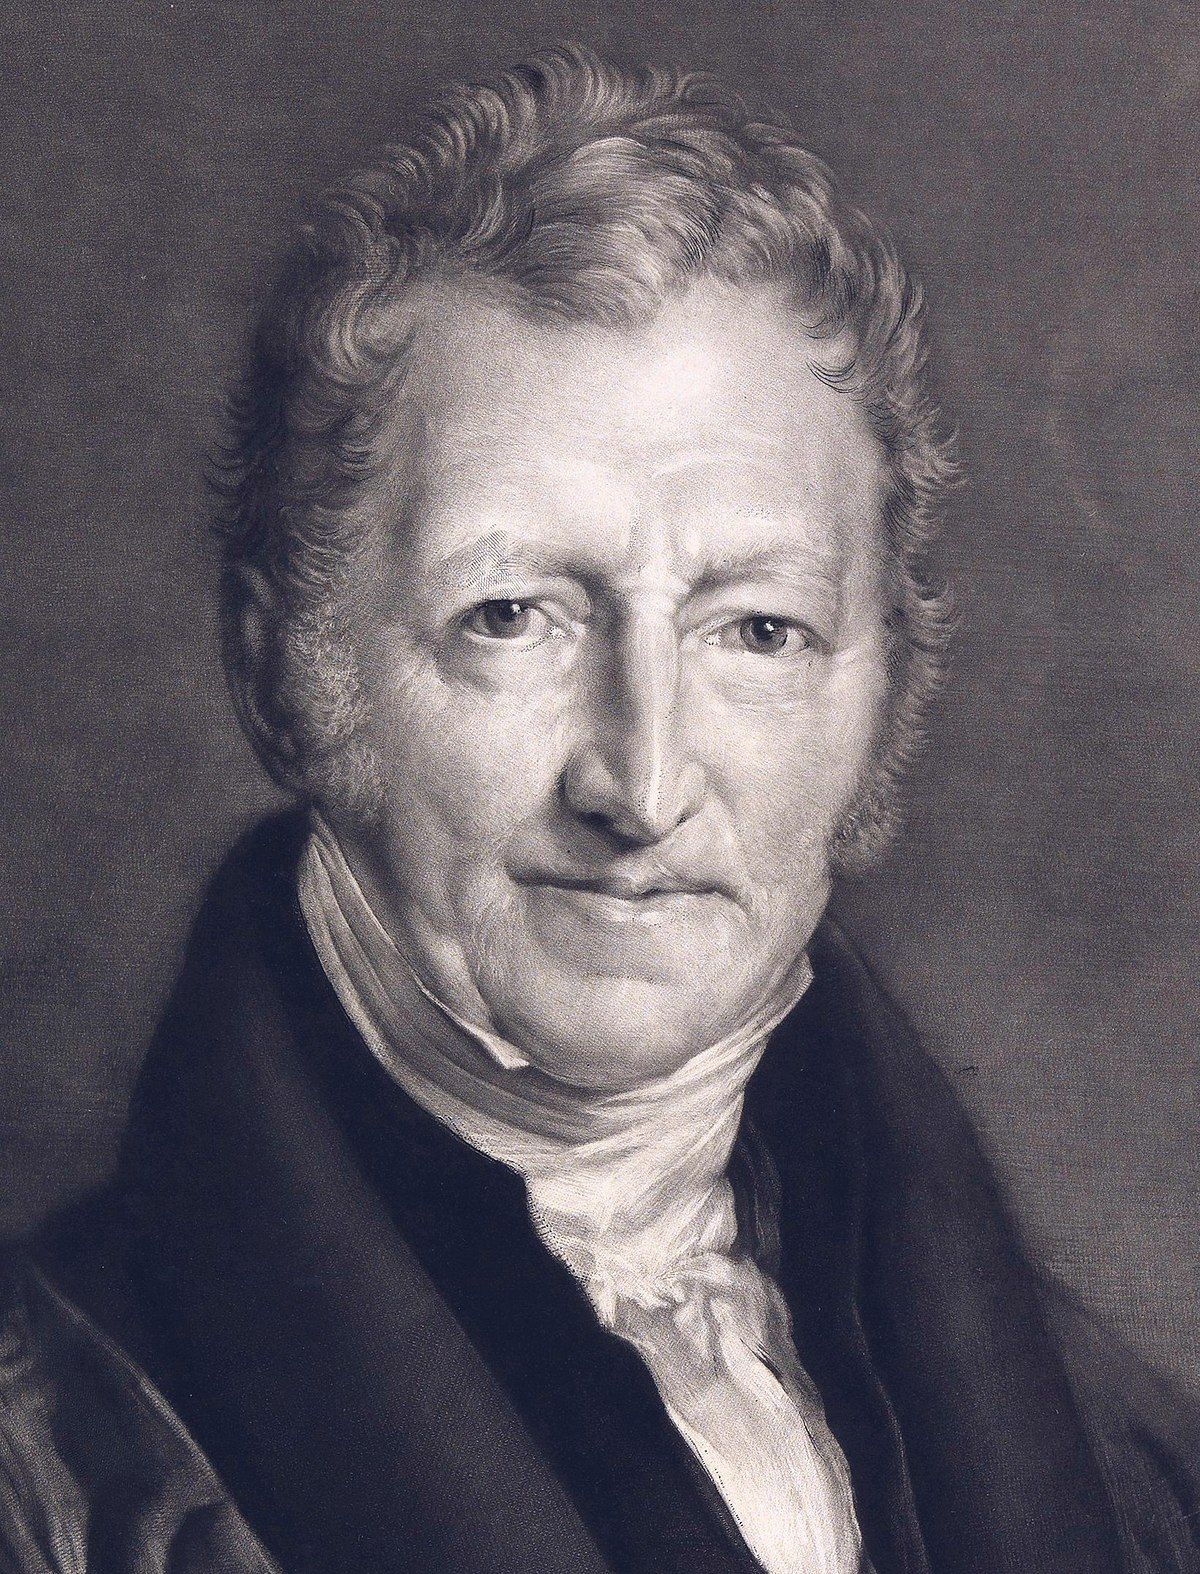
\includegraphics[scale=0.2]{assets/lectures_recent-44a47cac.png} \end{center}

Томас Мальтус (1766-1834), -- англійский вчений, демограф, економіст, священик; 1798 року: ''Все про принципи народонаселення.''
$$
\dfrac{\mathrm{d}x}{\mathrm{d}t} = ax \Longrightarrow x(t) = C \cdot e^{at} \text{ -- загальний розв'язок.}
$$
Нехай в початковий момент часу $t_0 = 0$ кількість особин складає $x_0$ особин:
$$
x(0) = x_0
$$
Тоді: $x(t) = x_0 \cdot e^{at} $ -- розв'язок даної задачі Коші. Розглянемо випадки:

\begin{enumerate}
  \item $a < 0$ (помирають більше, ніж народжується). Оскільки дане рівняння є лінійним, то всі розв'язки водночас стійкі (нестійкі, асимптотично стійкі). Тому дослідимо на стійкість розв'язок $ \varphi(t) = 0$ (умова 1. стійкості виконується); розв'язок довільної задачі Коші:
  $$
  x(t_0) = x_0 \quad : \quad x(t) = x_0 e^{a (t-t_0)}
  $$
  Нехай $ \left| x_0 \right| < \delta.$ Розглянемо:
  $$
  \forall t \geq t_0 \quad \left| x (t) \right| = \underbrace{e^{a(t-t_0)}}_{<1, \text{ при } t\geq t_0} \left| x_0 \right| \xrightarrow[t\to + \infty]{} 0 < \varepsilon \text{ при } \varepsilon = \delta
  $$
  $\Rightarrow $ всі розв'язки рівняння асимптотично стійкі та прямують до нуля.\\
  \begin{center} 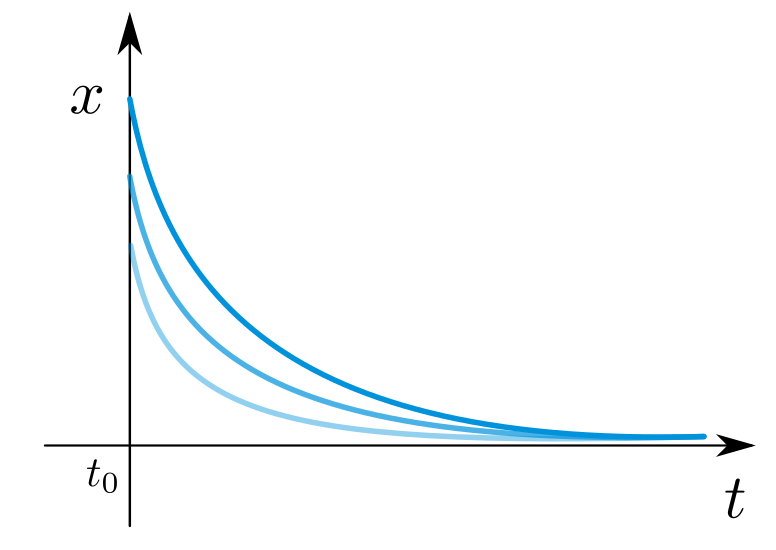
\includegraphics[scale=0.33]{assets/lectures_recent-562c17da.png} \end{center}
  Це означає, що якою б великою не була кількість особин в початковий момент часу, якщо смертність перевищує народжуваність, кількість особин з часом прямує до 0 ($t \to + \infty$).

  \item a = 0 (смертність = народжуваність). В цьому випадку розв'язок задачі Коші:
  $$ x(t_0) = x_0 \quad : \quad x(t) = x_ 0 $$
  Відповідно при $|x_0| < \delta$ маємо $|x(t)| = |x_0| < \varepsilon = \delta$. Отримали стійкість, але не асимптотичну.
  \begin{center}
    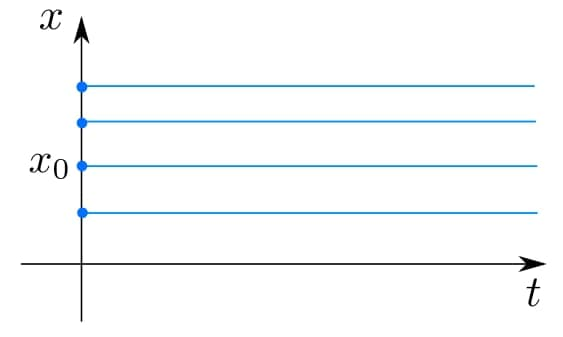
\includegraphics[scale=0.65]{assets/bcase.jpg}
  \end{center}
  Чисельність особин є сталою в кожний момент часу, коли смертність співпадає з народжуваністю.

  \item a > 0 (смертність < народжуваність). Візьмемо $\varphi(t) = 0$, розв'язок для будбудь-якої задачі Коші:
  $$ x(t_0) = x_0e^{a(t-t_0)}$$
  Нехай $|x_0| < \delta$
  $$\forall t \geq t_0 \quad |x(t)| = e^{a(t-t_0)}|x_0| \rightarrow +\infty \quad \text{ при } \quad t \rightarrow +\infty$$
  Отже,
  $$\exists \varepsilon > 0 \quad \exists t_0 \geq 0 : \forall \delta > 0$$ для розв'язку $x(t)$ з початковими умовами $x(t_0) = x_0 : |x(t_0)| < \delta$, але $|x(t)| > \varepsilon$, починаючи з деякого моменту (нестійкість)
  \begin{center}
    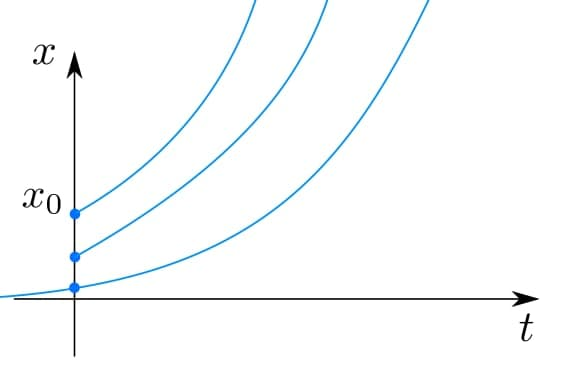
\includegraphics[scale=0.65]{assets/vcase.jpg}
  \end{center}
  В даному випадку чисельність особин необмежено, експоненційно зростає з часом і $\rightarrow +\infty$ при $t \rightarrow +\infty$, розв'язки рівняння нестійкі.
\end{enumerate}

\subsubsection{Модель Ферхюльста (логістична модель)}
\begin{center}
  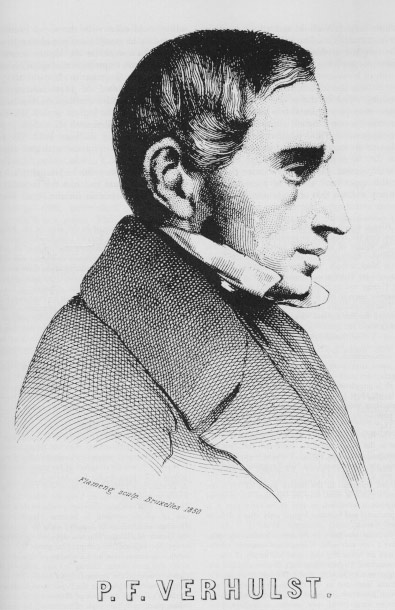
\includegraphics[scale=0.6]{assets/verhulst.jpg}
\end{center}

Нехай між особинами є внутрішньовидова боротьба, що додає додаткове джерело загибелі. Отже смертність:
\begin{enumerate}
  \item природна:  $-\sigma x$;
  \item внутрішньовидова боротьба: $- \mu x^2$.
\end{enumerate}

Швидкість народжуваності: $S = \gamma x$.  Швидкість смертності: $S = - \sigma x - \mu x^2$.\\
$$
\dfrac{\mathrm{d}x}{\mathrm{d}t}  = \gamma x -  \sigma x - \mu x^2 = \underbrace{(\gamma - \sigma)}_{=аеa}x - \mu x^2
$$

\begin{center}
    \fbox{$ \dfrac{\mathrm{d}x}{\mathrm{d}t} = ax - \mu x^2 $} -- закон Ферхюльста.
\end{center}
Розглянемо $a > 0$, тобто народжуваність більше смертності.
\begin{center}
  Зауважимо, що $ax - \mu x^2 = x ( a - \mu x)$.
\end{center}

Проаналізувавши праву частину, бачимо, що:
\begin{itemize}
  \item $\dfrac{\mathrm{d}x}{\mathrm{d}t} > 0 (\uparrow) \text{ при } x \in (0, \dfrac{a}{\mu})$
  \item $\dfrac{\mathrm{d}x}{\mathrm{d}t} < 0 (\downarrow) \text{ при } x \in (- \infty, 0) \cup ( \dfrac{a}{\mu}, +\infty)$
  \item $\dfrac{\mathrm{d}x}{\mathrm{d}t} = 0 \text{ при } x = 0 \lor x = \dfrac{a}{\mu}$
\end{itemize}

\begin{center} 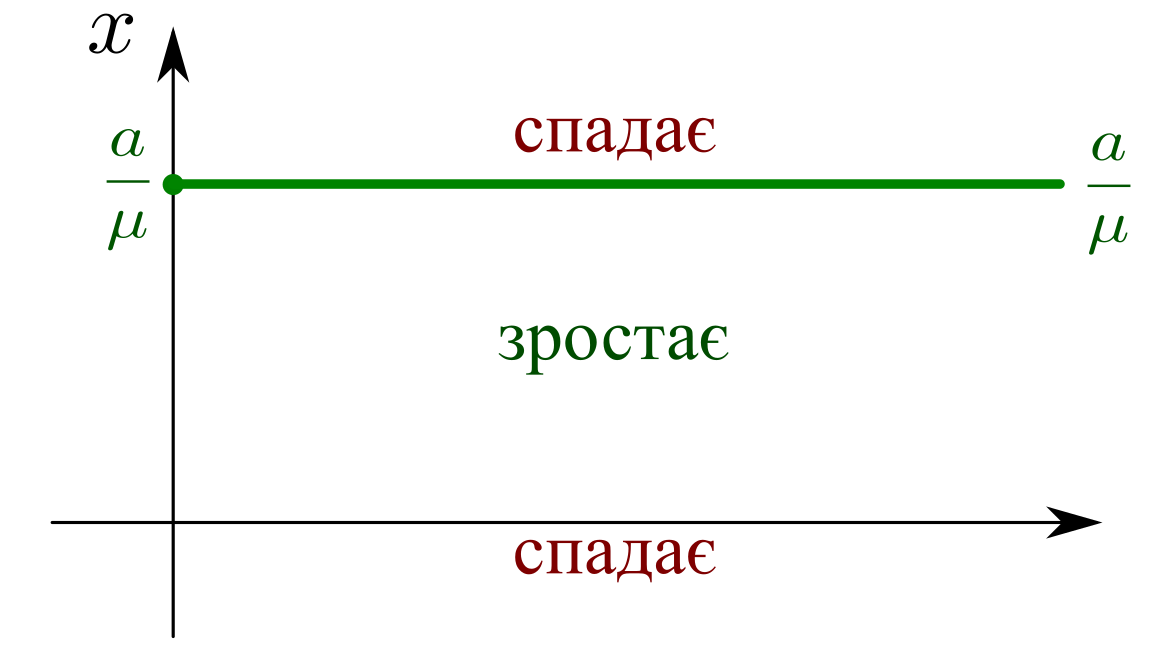
\includegraphics[scale=0.28]{assets/lectures_recent-e4b7cd02.png} \end{center}

Розв'яжемо рівняння: $\dfrac{\mathrm{d}x}{\mathrm{d}t} = ax - \mu x^2 $ -- рівняння Бернуллі.
\begin{spacing}{2}
  $x = u\cdot v $, $ \quad u'v + v'u - auv = - \mu u^2 v^2 $, $\quad u'v + u(v' - av) = - \mu u^2 v^2 $\\
  $v' = av$, $\quad \dfrac{\mathrm{d}v}{v} = a\mathrm{d}t \quad \Longrightarrow \quad v = e^{at}$, $\quad u' =- \mu u^2 v$, $\quad \dfrac{\mathrm{d}u}{u^2} = - \mu e^{at}\mathrm{d}t $\\
  Тоді: $ -\dfrac{1}{u} = -\dfrac{ \mu}{a}e^{at} - C $, звідси отримуємо:\\
  $ u = \dfrac{1}{ \frac{u}{a} e^{at} +c } = \dfrac{a}{ \mu e^{at} + aC} \quad \Longrightarrow \quad x = uv = \dfrac{a e^{at}}{ \mu e^{at} + aC  }  =  \dfrac{a}{ \mu  + aCe^{-at}}  $\\ \\
  Загальний розв'язок:
  $\left[ \begin{gathered}
   x= \frac{a}{ \mu  + aCe^{-at}}\\
   x = 0
  \end{gathered} \right.$
\end{spacing}


Знайдемо довільний розв'язок задачі Коші: $x(t_0) = x_0: \quad x_0 = \dfrac{a}{\mu + aCe^{-at_0}}$\\
$\mu + aC\cdot e^{-at_0} = \dfrac{a}{x_0}, \quad C = \dfrac{\left( \dfrac{a}{x_0} - \mu  \right)\cdot e^{at_0} }{a} = \dfrac{a - \mu x_0}{ax_0}\cdot e^{at_0} \Longrightarrow$
$$
\Longrightarrow x(t) = \dfrac{a}{ \mu + \frac{a - \mu x_0}{x_0} \cdot e^{a(t_0 - t)} } = \dfrac{ax_0}{ \mu x_0 - (a - \mu x_0 ) \cdot e^{a(t_0-t)}}
$$

Отримали розв'язок $ \varphi (t) = \dfrac{a}{\mu} \quad \exists $  на $[0, + \infty)$.
\begin{spacing}{3}
  Перевіримо другу умову стійкості. Візьмемо $ \left| x - \dfrac{a}{\mu} \right| = \left| \dfrac{\mu x_0 - a}{\mu}  \right| < \delta $
  \\ і розглянемо: $
  \left| x(t) - \varphi(t) \right| = \left| \dfrac{ax_0}{\mu x_0 - (a - \mu x_0) \cdot e^{a (t_0 - t)}}  - \dfrac{a}{ \mu}  \right| = \\ \left| \dfrac{a\mu x_0 - a\mu x_0 + a (a - \mu x_0 )\cdot e^{a(t_0 - t)}}{\mu (\mu x_0 - (a- \mu x_0)\cdot e^{a(t_0 -t)})}  \right| = \dfrac{a (a - \mu x_0)\cdot e^{a (t_0 - t)}}{ \mu^2 x_0 - \mu (a- \mu x_0) \cdot e^{a(t_0 - t)}} \xrightarrow[t\to +\infty]{} 0$
\end{spacing}


Таким чином, розв'язок $\varphi(t) = \frac{a}{\mu}$ - асимптотично стійкий.
\begin{center} 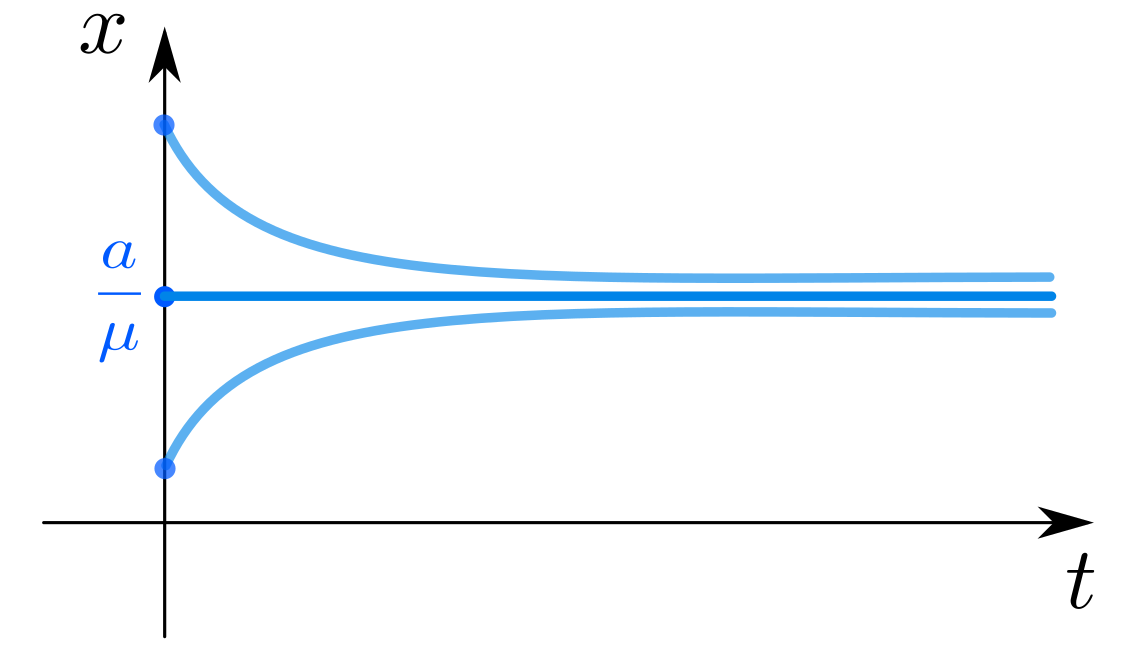
\includegraphics[scale=0.3]{assets/lectures_recent-0b98e3f0.png} \end{center}
\begin{remark}
    1. Аналогічно можна показати, що $\varphi (t) = 0$ - нестійкий. Таким чином, внутрішньовидова боротба виступає ''природнім стабілізатором'' моделі одновимірної популяції. На відміну від моделі Мальтуса, де у випадку $ a > 0$ маємо нестійкість і нескінчений ріст популяції, в моделі Ферхюльста розв'язки стабілізуються в околі стлого розв'язку $\varphi(t) = \dfrac{a}{\mu}.$ Відзначимо також, що чим меньше значення $\mu$, тим швидше зростає чисельність особин.
\end{remark}
\begin{remark}
    2. При $ a\leq 0$ (смертність $\geq$  народжуваність) легко встановити, що $ x=0 $ -- асимптотично стійкий розв'язок.
\end{remark}

\subsection{Класифікація фазових портретів в околі положень рівноваги ЛОС 2-го порядку.}

\begin{defo}
    Положенням рівноваги нормальної системи диф. рівнянь:
    $$
    \begin{dcases}
        \dot{x_1} = f_1(x_1, ..., x_n)\\
        \qquad \quad \cdots\\
        \dot{x_n} = f_n(x_1, ..., x_n)
    \end{dcases}
    $$
    називається т. $\overline{x} = (x_1, ... , x_n)$ така, що:
    $$
    f_1 (\overline{x}) = f_2(\overline{x}) = \cdots = f_n(\overline{x}) =0
    $$
\end{defo}
Розглянемо ЛОС (1):$ \begin{cases}
    \dot{x} = ax + by\\
    \dot{y} = cx + dy
\end{cases}$, $\quad$ де a, b, c, d $\in \mathbb{R}, \quad A = \begin{bmatrix}
 a & b\\
 c & d
\end{bmatrix}$.\\


Нехай $\det A \neq 0$. Тоді єдине положення рівноваги системи (1) -- це точка (0,0).
\begin{defo}
    Фазовою траєкторією ЛОС (1) називається проекція її інтегральних кривих на площину $xOy$. Зображення фазових траєкторій на площині $xOy$ називають фазовим портретом.
\end{defo}
\textbf{Завдання.} Дослідити фазовий портрет ЛОС (1) в околі т. (0, 0), яка є її положенням рівноваги. Виявляється, що фазовий портрет ЛОС (1) в околі точки (0, 0) повністю визначається власними числами матриці $A$. Нехай $J(A)$ -- ЖНФ матриці $A$; $H$ - матриця переходу. \\

1. Нехай $\lambda_1 , \lambda_2 \in \mathbb{R} \quad \lambda_1 \neq \lambda_2 \quad \lambda_1 \cdot \lambda_2 > 0.$ \\ Для зручності здійснимо в системі (1):

$$
\begin{bmatrix}
 \dot{x}\\
 \dot{y}
\end{bmatrix} = A \begin{bmatrix}
 x \\
 y
\end{bmatrix} \text{ заміну: } \begin{bmatrix}
 x\\
 y
\end{bmatrix} = H \begin{bmatrix}
 u \\ v
\end{bmatrix} \text{, де }
 \begin{bmatrix}
 u \\
 v
\end{bmatrix} \text{ -- нова невідома вектор-функція}
$$

$$
H \begin{bmatrix}
 \dot{u}\\
 \dot{v}
\end{bmatrix} = A H  \begin{bmatrix}
 u \\
 v
\end{bmatrix} \quad \text{домножимо зліва на } H^{-1} \text{, тоді: }
H^{-1} H \begin{bmatrix}
\dot{u}\\
\dot{v}
\end{bmatrix}  =H^{-1} A H \begin{bmatrix}
 u \\
 v
\end{bmatrix}
$$

$$ \text{Таким чином, ми перейшли до Жарданового базису: }
\begin{bmatrix}
\dot{u}\\
\dot{v}
\end{bmatrix}  =J(A) \cdot \begin{bmatrix}
 u \\
 v
\end{bmatrix}
$$
Маємо: $ \begin{bmatrix}
\dot{u}\\
\dot{v}
\end{bmatrix} = \begin{bmatrix}
 \lambda_1 & 0 \\
 0 & \lambda_2
\end{bmatrix} \begin{bmatrix}
 u \\
 v
\end{bmatrix}$




$$
\left[ \begin{array}{l}
    \dfrac{dv}{du} = \dfrac{\lambda_2}{\lambda_1} \cdot \dfrac{u}{v}\\
    u = 0
\end{array} \right.
\Longleftarrow
\begin{cases}
    \dot{u} = \lambda_1 u \\
    \dot{v} = \lambda_2 v
\end{cases} \Longrightarrow
\begin{cases}
    u = c_1 \cdot e^{\lambda_1 t}\\
    v = c_2 \cdot e^{\lambda_2 t}
\end{cases}
$$
Поділили двуге рівняння на перше, щоб вилучити $t$.
$$
\left[ \begin{array}{l}
    \dfrac{dv}{du} = \dfrac{\lambda_2}{\lambda_1} \cdot \dfrac{u}{v}\\
    u = 0
\end{array} \right. \Longrightarrow \left[ \begin{array}{l}
    \ln{ \left| v \right| } = \dfrac{\lambda_2}{\lambda_1} \ln{ \left| u \right| } + \ln{ \left| c \right| } \\
    u = 0, v = 0
\end{array} \right. \Longrightarrow
\left[ \begin{array}{l}
    v = c  \cdot u^{ \frac{\lambda_2}{\lambda_1} }\\
    u = 0, v = 0
\end{array} \right.
$$

Якщо $ \lambda_1 \cdot \lambda_1 > 0 $ та $ \left| \lambda_2 \right| > \left| \lambda_1 \right|  $ (стрілки від нуля за умови $
 \lambda_1, \lambda_2 > 0$):

\begin{center} 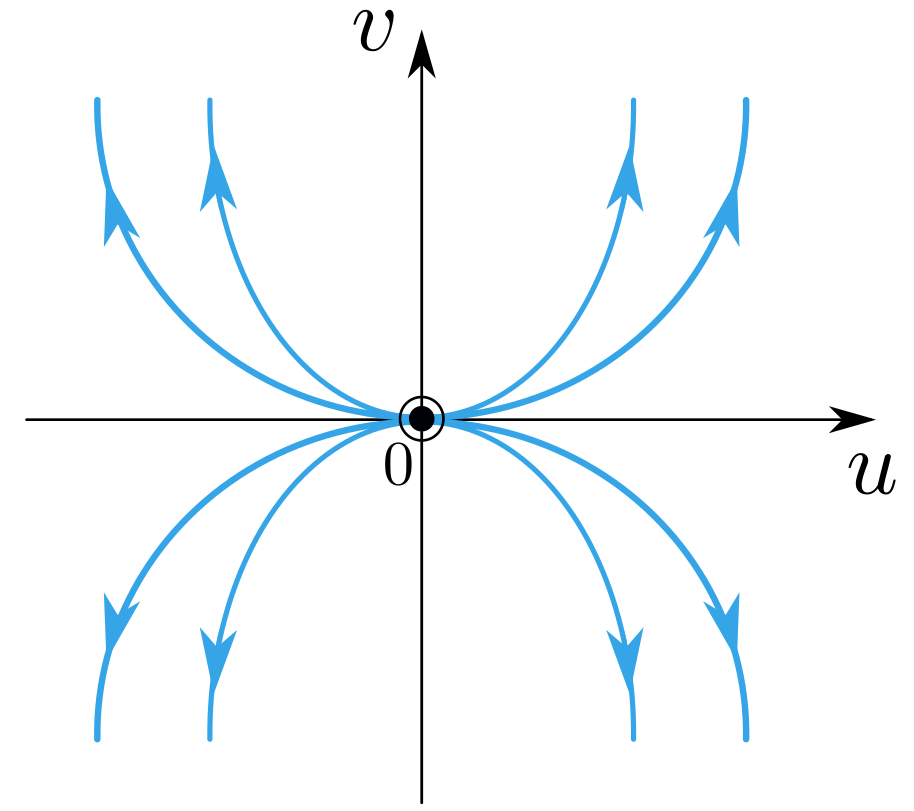
\includegraphics[scale=0.3]{assets/lectures_recent-b13d607a.png} \end{center}

Якщо $ \lambda_2 \cdot \lambda_1 > 0$ та  $ \left| \lambda_2 \right| > \left| \lambda_1 \right|  $ (стрілки до нуля за умови $
 \lambda_1, \lambda_2 < 0$):

 \begin{center} 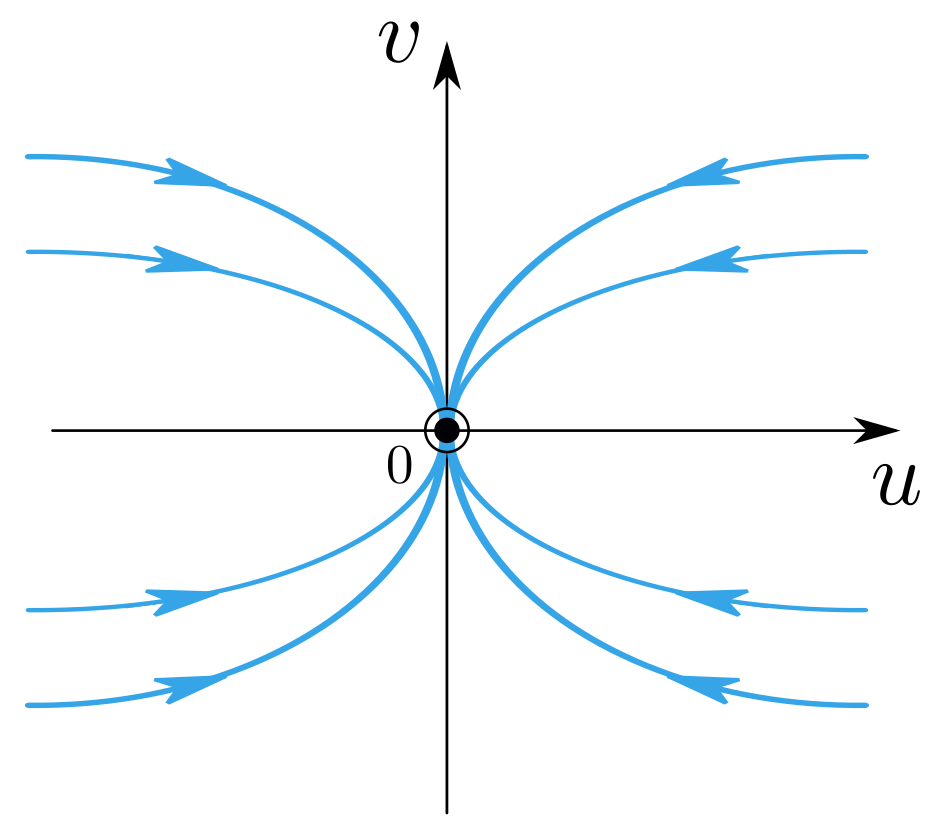
\includegraphics[scale=0.3]{assets/lectures_recent-392ff5ad.png} \end{center}

 Відмітимо, що якщо $\lambda_1, \lambda_2 < 0$, то напрям руху (по $t$) вздовж траєкторій відбувається до нуля. Якщо ж $\lambda_1, \lambda_2 >0$, то рух спрямовано від нуля.\\

 Залишається перейти до початкових змінних $ \begin{bmatrix}
  x \\
   y
 \end{bmatrix}$.\\
Таким чином, якщо $\lambda_1 , \lambda_2 \in \mathbb{R}, \lambda_1 \neq \lambda_2, \lambda_1 \cdot \lambda_2 > 0$ (власні числа одного знаку), то фазовий портрет має вигляд:

\begin{center} 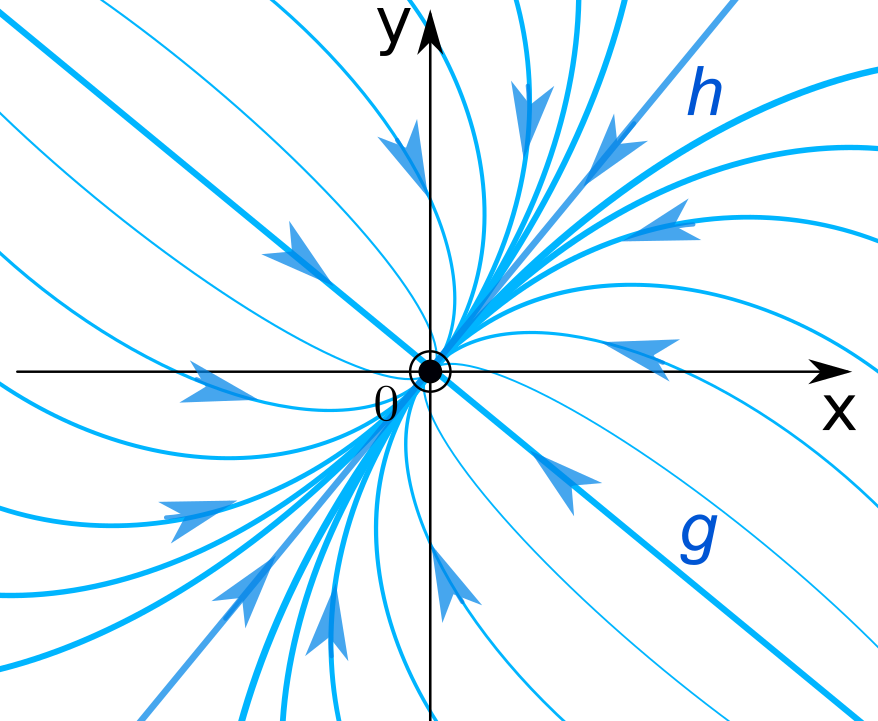
\includegraphics[scale=0.3]{assets/lectures_recent-deaf1762.png} \end{center}

На малюнку $h$ - пряма на якій лежить власний вектор, який відповідає меншому за модулем власному числу.\\
Такий фазовий портрет \textbf{вузол.}\\
- Якщо $\lambda_1, \lambda_2 > 0$ - нестійкий вузол (стрілки від нуля).\\
- Якщо $\lambda_1, \lambda_2 < 0$ - ас. стійкий вузол (стрілки до нуля).

\begin{example}
    $$
    \begin{cases}
    \dot{x} = 2y - 3x\\
    \dot{y} = x - 4y
    \end{cases} \qquad A = \begin{bmatrix}
     -3 & 2 \\
     1 & -4
    \end{bmatrix}
    $$
    $$
    \det{A - \lambda I} = \begin{vmatrix}
      -3 - \lambda & 2 \\
      1 & -4 - \lambda
    \end{vmatrix}  = (-3-\lambda) (-4 - \lambda) -2 = \lambda^2 + 7 \lambda + 10 = 0
    $$
    $$
    \lambda_1 = -2 \qquad \lambda_2 = -5 \Rightarrow \text{ас. стійкий вузол.}
    $$
    Знаходимо власні вектори:\\
    $\lambda_1 = -2$:
    $$
    \begin{bmatrix}
     -1 & 2 \\
     1 & -2
    \end{bmatrix} \begin{bmatrix}
     h_1 \\
     h_2
    \end{bmatrix} = \begin{bmatrix}
     0 \\
     0
    \end{bmatrix} \qquad \begin{gathered}
     -h_1 + 2h_2 = 0\\
     h_1 = 2 h_2
    \end{gathered} \Rightarrow \overline{h} = \begin{bmatrix}
     2 \\
     1
    \end{bmatrix}
    $$
    $\lambda_2 = -5$
    $$
    \begin{bmatrix}
     2 & 2 \\
     1 & 1
    \end{bmatrix} \begin{bmatrix}
     g_1 \\
     g_2
    \end{bmatrix} = \begin{bmatrix}
     0 \\
     0
    \end{bmatrix}
    \qquad \begin{gathered}
     g_1 + g_2 = 0\\
     g_1 = - g_2
    \end{gathered} \Rightarrow \overline{g} = \begin{bmatrix}
     1 \\
     -1
    \end{bmatrix}
    $$

    \begin{center} 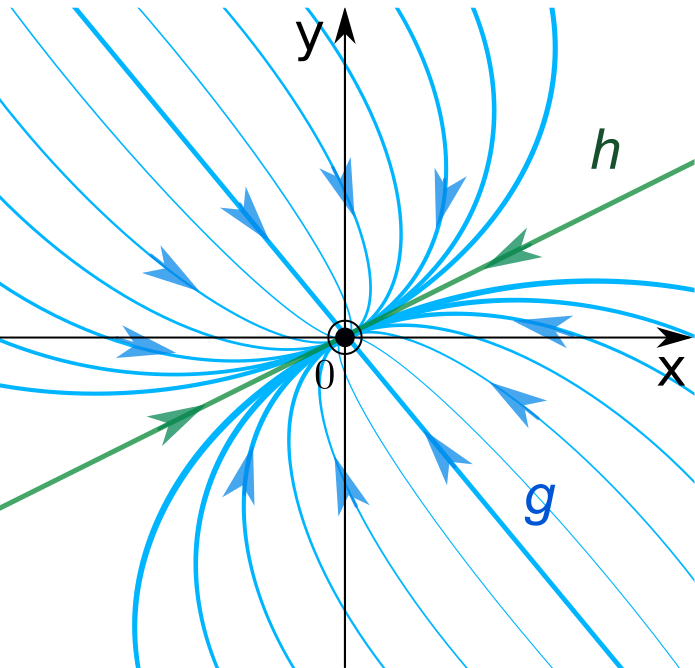
\includegraphics[scale=0.4]{assets/lectures_recent-06adae22.png} \end{center}
\end{example}

2. Нехай $ \lambda_1 , \lambda_2 \in \mathbb{R}, \lambda_1 \neq \lambda_2, \lambda_1 \cdot \lambda_2 < 0$ (Власні числа різних знаків).
Тоді, аналогічно, перейшовши до Жорданового базису, маємо:

$$
\begin{gathered}
\begin{cases}
    \dot{u} = \lambda_1 u\\
    \dot{v} = \lambda_2 v
\end{cases} \\ \begin{cases}
    u = c_1 \cdot e^{\lambda_1 t}\\
    v = c_2 \cdot e^{\lambda_2 t}
\end{cases} \\
 \left[ \begin{array}{l}
v = C \cdot u^{ \frac{\lambda_2}{\lambda_1} }\\
u =0 , v = 0
\end{array} \right.
\end{gathered}\quad
\begin{gathered} 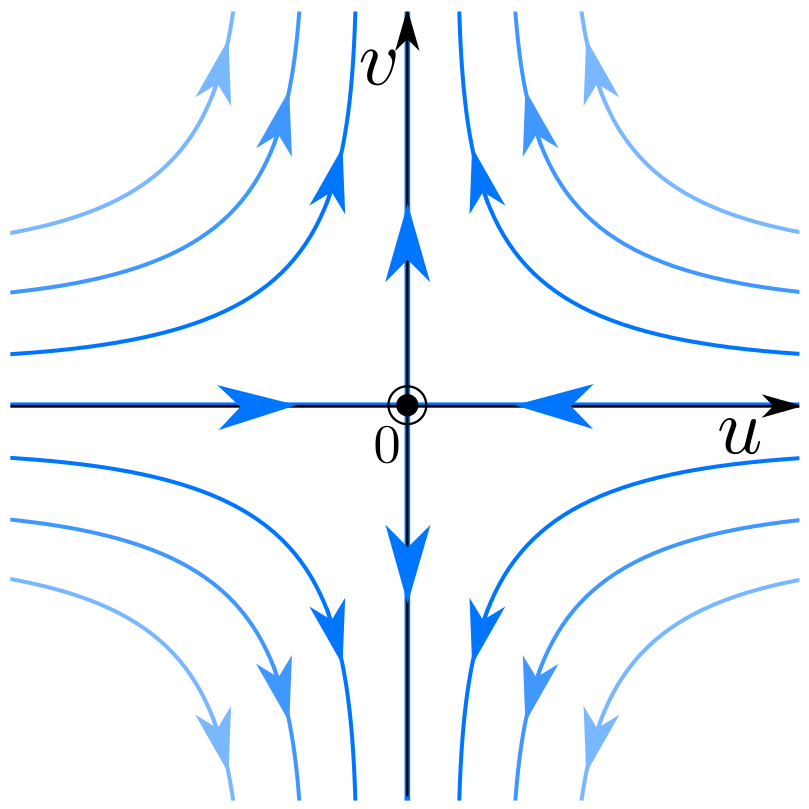
\includegraphics[scale=0.3]{assets/lectures_recent-53a0acd8.png} \end{gathered}
$$


Якщо $ \lambda_1 < 0,
  \lambda_2 > 0
$, то $
 \begin{gathered}
 u(t) \xrightarrow[t \to \infty]{} 0\\
 v(t) \xrightarrow[t \to \infty]{} \infty
 \end{gathered}.$\\
 Якщо $ \lambda_1 < 0,
  \lambda_2 > 0$, то  $
   \begin{gathered}
   u(t) \xrightarrow[t \to \infty]{} \infty\\
   v(t) \xrightarrow[t \to \infty]{} 0
   \end{gathered}.$\\
У другому випадку напрям руху траекторій відбуватиметься в інший бік.\\
Отже, перейшовши до початкових змінних, отримаємо, що за умови $\lambda_1 \cdot \lambda_2 < 0$ фазовий портрет має вигляд:

\begin{center} 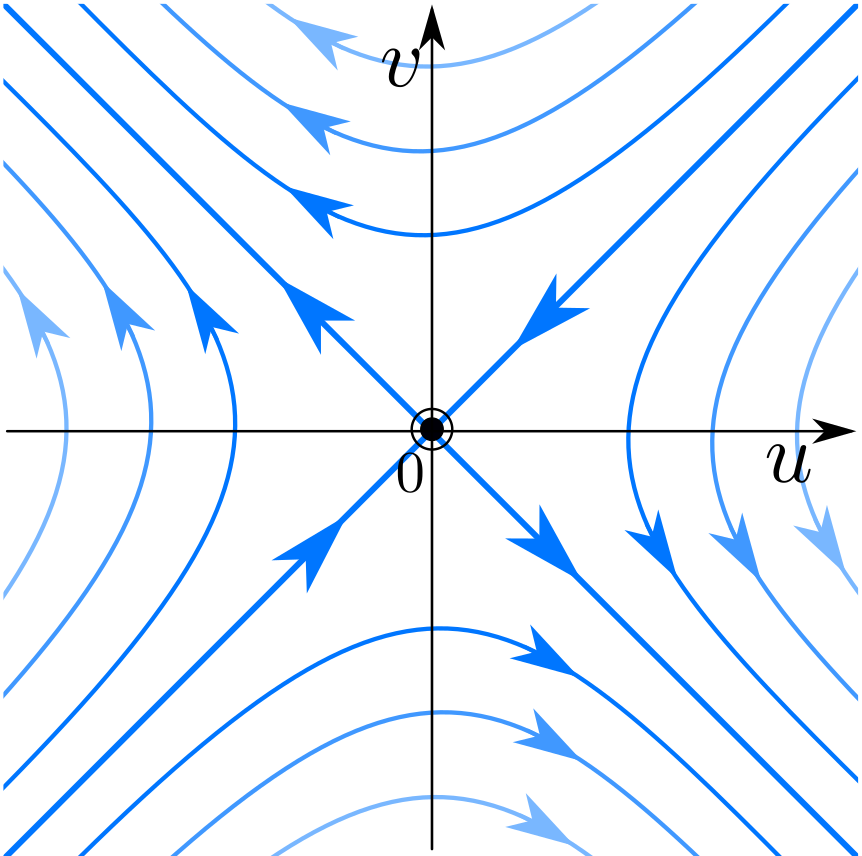
\includegraphics[scale=0.25]{assets/lectures_recent-0ebe704d.png} \end{center}

\begin{remark}
    Стрілки до нуля вздовж прямої, на якій лежить власний вектор, що відповідає $ \lambda_1 < 0$.\\
    Стрілки від нуля вздовж прямої, на якій лежить власний вектор, що відповідає $ \lambda_2 > 0$.
\end{remark}
Такий фазовий портрет називається \textbf{сідло}. Це завжди нестійке положення рівноваги.

\begin{example}
    $$
    \begin{cases}
        \dot{x} = x + 3y\\
        \dot{y} = 2x
    \end{cases} \qquad A = \begin{bmatrix}
     1 & 3 \\
     2 & 0
    \end{bmatrix}
    $$
    $$
    \det (A - \lambda I) = \begin{vmatrix}
      1-\lambda & 3 \\
      2 & - \lambda
    \end{vmatrix} = (1- \lambda)(-\lambda) - 6 = \lambda^2 - \lambda - 6 = 0
    $$
    $$
    \lambda_1 = 3 \quad \lambda_2 = -2 \Longrightarrow \text{сідло (нестійке)}
    $$
    Знаходимо власні вектори:
    $\lambda_1 = 3$
    $$
    \begin{bmatrix}
     -2 & 3\\
     2 & -3
    \end{bmatrix} \begin{bmatrix}
     h_1\\
     h_2
    \end{bmatrix} = \begin{bmatrix}
      0\\
      0
    \end{bmatrix} \qquad 2h_1 = 3 h_2 \Rightarrow \overline{h} = \begin{bmatrix}
     3 \\
     2
    \end{bmatrix}
    $$

    $\lambda_2 = -2$

    $$
    \begin{bmatrix}
     3 &3 \\
     2 & 2
    \end{bmatrix} \begin{bmatrix}
     g_1 \\
     g_2
    \end{bmatrix} = \begin{bmatrix}
     0 \\
     0
    \end{bmatrix} \qquad 2 g_1 =-2 g_2 \Rightarrow \overline{g} = \begin{bmatrix}
     1 \\
     -1
    \end{bmatrix}
    $$
    Отримали такий фазовий портрет:
    \begin{center} 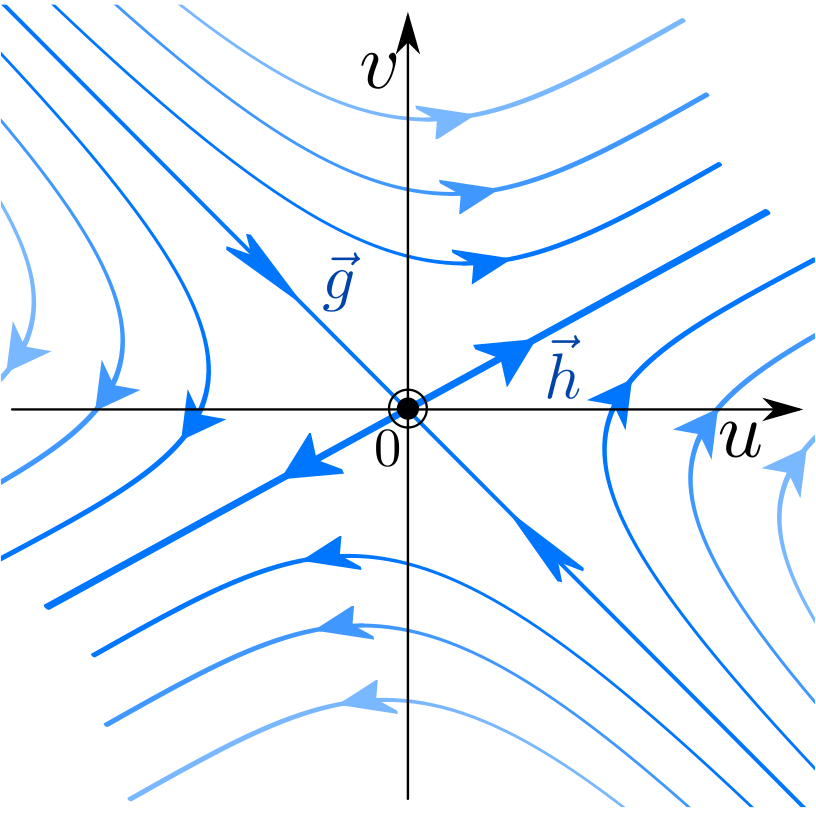
\includegraphics[scale=0.3]{assets/lectures_recent-c4b9c37b.png} \end{center}
    \end{example}


    3. Нехай $ \lambda_1 = \lambda_2 = \lambda \in \mathbb{R}$.\\
    a) Матриця $A$ - діагональна.
    $$
    A = \begin{bmatrix}
     \lambda & 0 \\
     0 & \lambda
    \end{bmatrix} \Longrightarrow \begin{cases}
        \dot{x} = \lambda x\\
        \dot{y} = \lambda y
    \end{cases}
    $$
    В такому випадку, фазовий портрет називають \textbf{диктричний вузол.}




\begin{center} 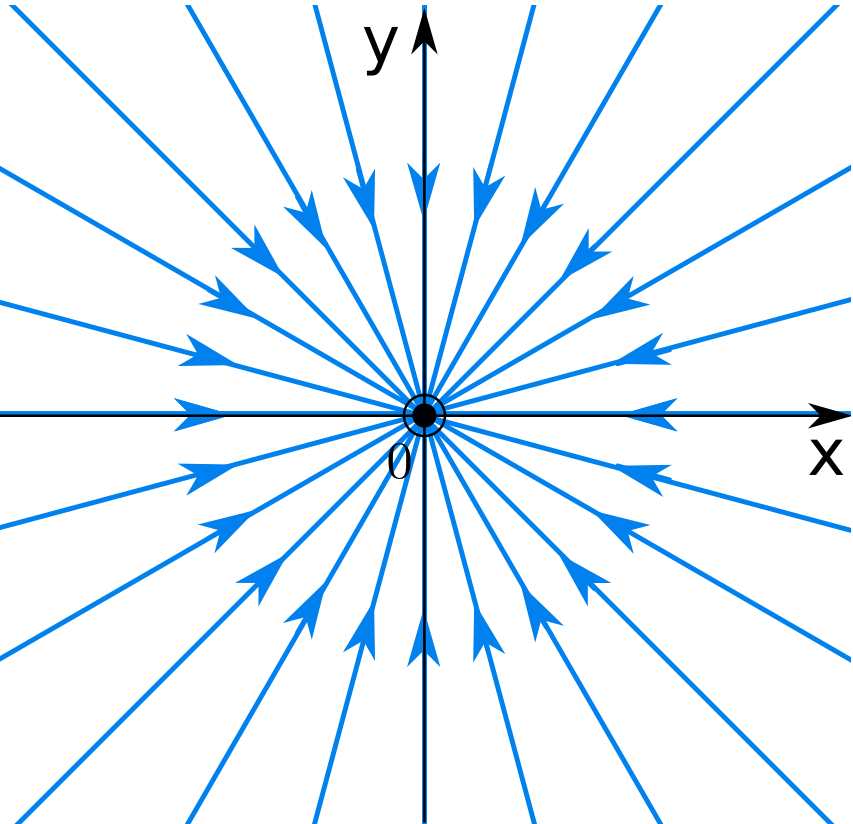
\includegraphics[scale=0.3]{assets/lectures_recent-ab36e3f3.png} \end{center}


Якщо $ \lambda < 0 $ - ас. стійкий (стрілки до нуля).\\
Якщо $ \lambda > 0 $ - нейстійкий (стрілки від нуля). \\
б) Матриця $A$ - недіагональна. В такому разі, фазовий портрет називають \textbf{вироджений вузол.}\\
- якщо $ \lambda < 0 $ - ас. стійкий ( стрілки до нуля ).\\
- якщо $ \lambda > 0 $ - нестійкий (стрілки від нуля).\\
Вироджений вузол може бути двох видів:
\begin{center} 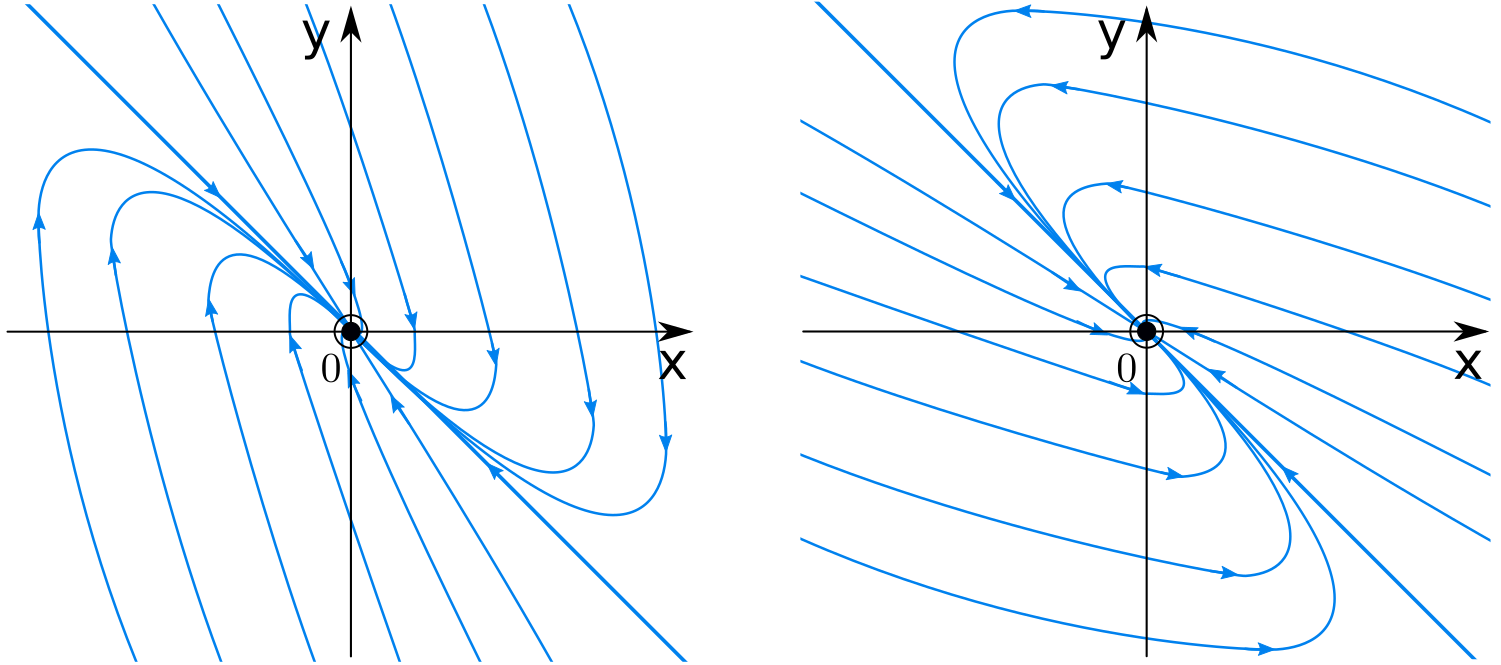
\includegraphics[scale=0.25]{assets/lectures_recent-b526bf37.png} \end{center}

Для визначення типу виродженого вузла потрібно визнгачити напрям вектора фазової швидкості $ \begin{bmatrix}
 \vec{x} \\
 \vec{y}
\end{bmatrix}$ в довільній точці, що не дорівнює нулю системи координат. Цей напрям має співпадати із напрямами руху по фазовій траєкторії (до нуля або від нуля).

\begin{example}
    $$
    \begin{cases}
        \vec{x} = 2y - 3x\\
        \vec{y} = y - 2x
    \end{cases} \qquad A = \begin{bmatrix}
     -3 & 2 \\
     -2 & 1
    \end{bmatrix}
    $$

    $$
    \det{ \left( A - \lambda I  \right) } = \begin{vmatrix}
      -3 - \lambda & 2 \\
      -2 & 1 - \lambda
    \end{vmatrix} = ( -3 - \lambda ) ( 1 -\lambda) + 4 =  \lambda^2 + 2 \lambda + 1 =
    $$
    $$
    = ( \lambda+ 1) ^2 = 0 \Longrightarrow  \lambda = -1 - \text{кратності 2. }
    $$
З попереднього випливає, що фазовим портретом буде асимптотично стійкий вироджений вузол (стрілки до нуля).
Знайдемо власний вектор:
$$
\begin{bmatrix}
 -2 & 2 \\
 2 & 2
\end{bmatrix} \begin{bmatrix}
 h_1 \\
 h_2
\end{bmatrix} = \begin{bmatrix}
 0 \\
 0
\end{bmatrix} \qquad h_1 = h_2 \Rightarrow \overline{h} = \begin{bmatrix}
 1 \\
 1
\end{bmatrix}
$$

\begin{center} 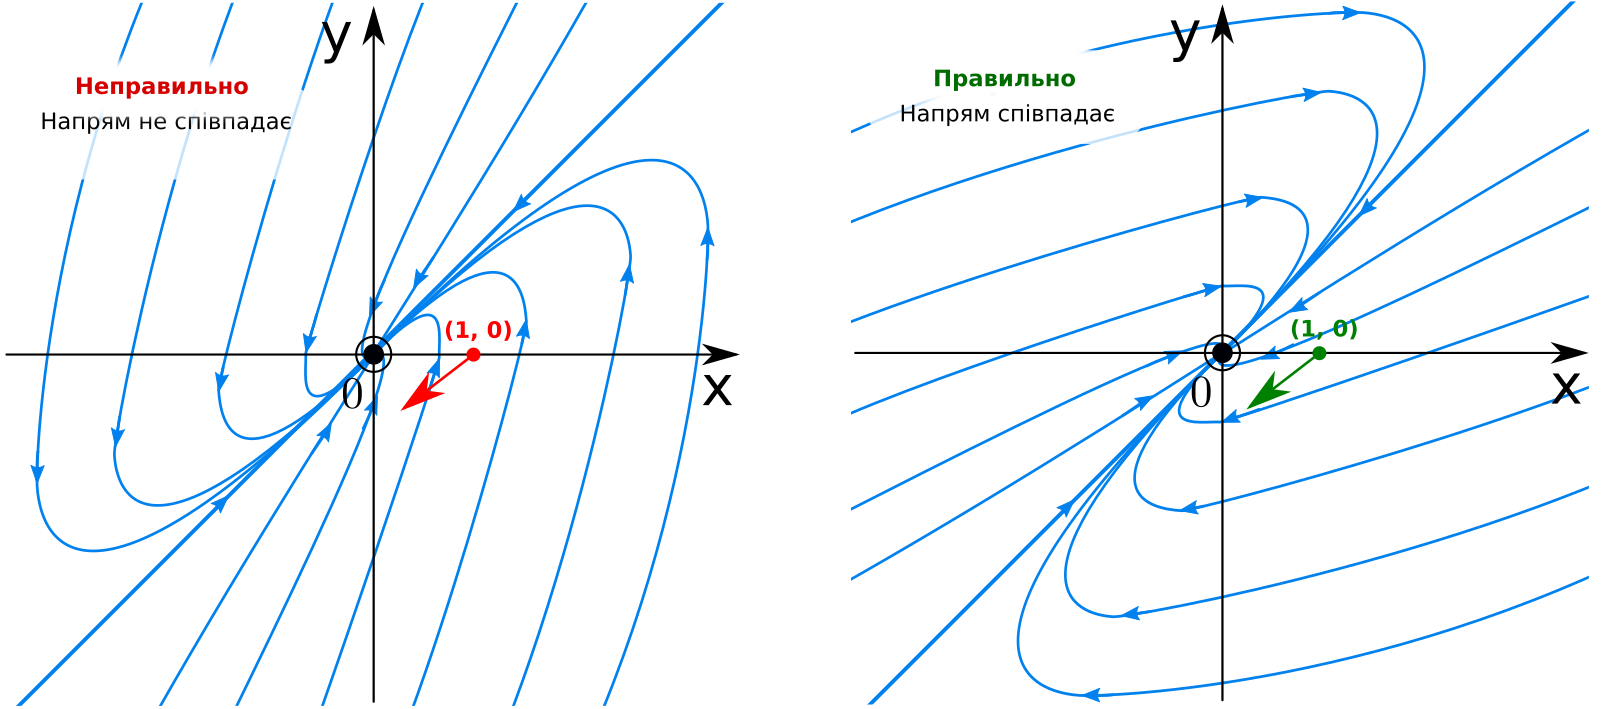
\includegraphics[scale=0.3]{assets/lectures_recent-f0de3cfc.png} \end{center}

Візьмемо т. (1, 0):
$$
\begin{bmatrix}
 \dot{x} \\
 \dot{y}
\end{bmatrix} \Bigg|_{(1,0)} = \begin{bmatrix}
 -3 \\
 -2
\end{bmatrix} \Longrightarrow \begin{gathered}
 x_k = -2 \\
 y_k = -2
\end{gathered}
$$

\end{example}

4. $\lambda_{1, 2} - \alpha \pm i\beta, \alpha\neq 0$. В такому випадку, фазовий портрет назвається \textbf{фокус}. Якщо $ \alpha > 0$ - нестійкий. Якщо $ \alpha > 0$ - ас. стійкий.
Фазовий портрет ''фокус'' може бути двох видів:
\begin{center} 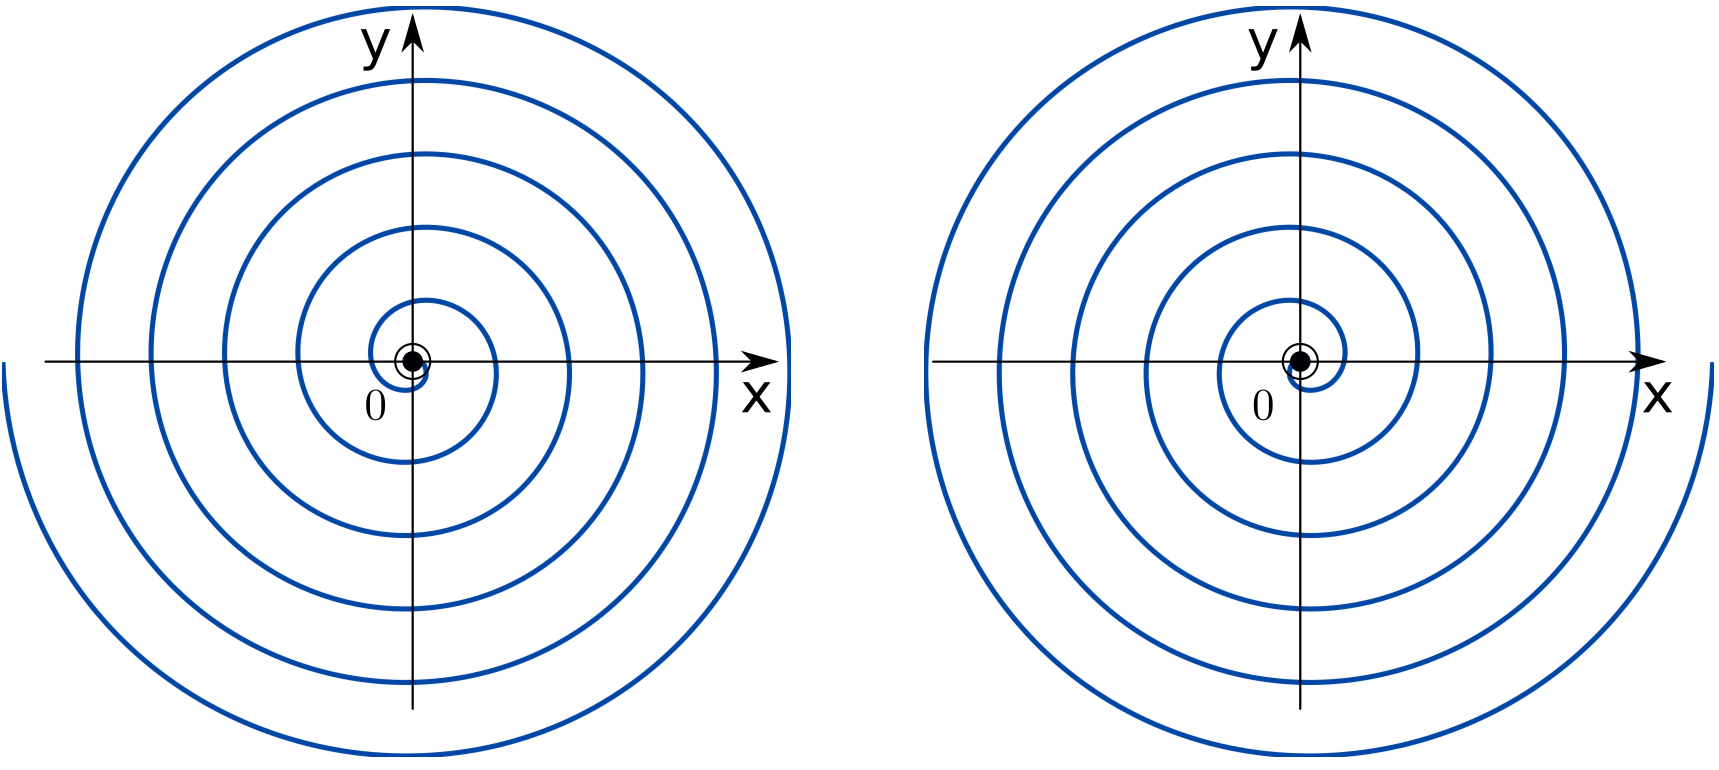
\includegraphics[scale=0.3]{assets/lectures_recent-9fe11a21.png} \end{center}
Для визначення типу фокуса визначаємо напрям вектора фазової швидкості в довільній точці, що не дорівнює нулю.

\begin{example}
    $$
    \begin{cases}
        \dot{x } = x - 2y\\
        \dot{y} = 4x - 3y
    \end{cases} \qquad A = \begin{bmatrix}
     1 & -2 \\
     4 & -3
    \end{bmatrix}
    $$
    $$ \det{(A - \lambda I)} = \begin{vmatrix}
      1- \lambda & -2 \\
      4 & -3-\lambda
    \end{vmatrix}  = ( 1- \lambda) (-3 - \lambda) + 8 = \lambda^2 + 2 \lambda + 5 = 0$$
$$
D = -16 \quad \lambda_{1,2} = \frac{-2 \pm 4i}{2} = -1 \pm 2i
$$
Асимптотично стійкий фокус (стрілки до нуля).
\begin{center} 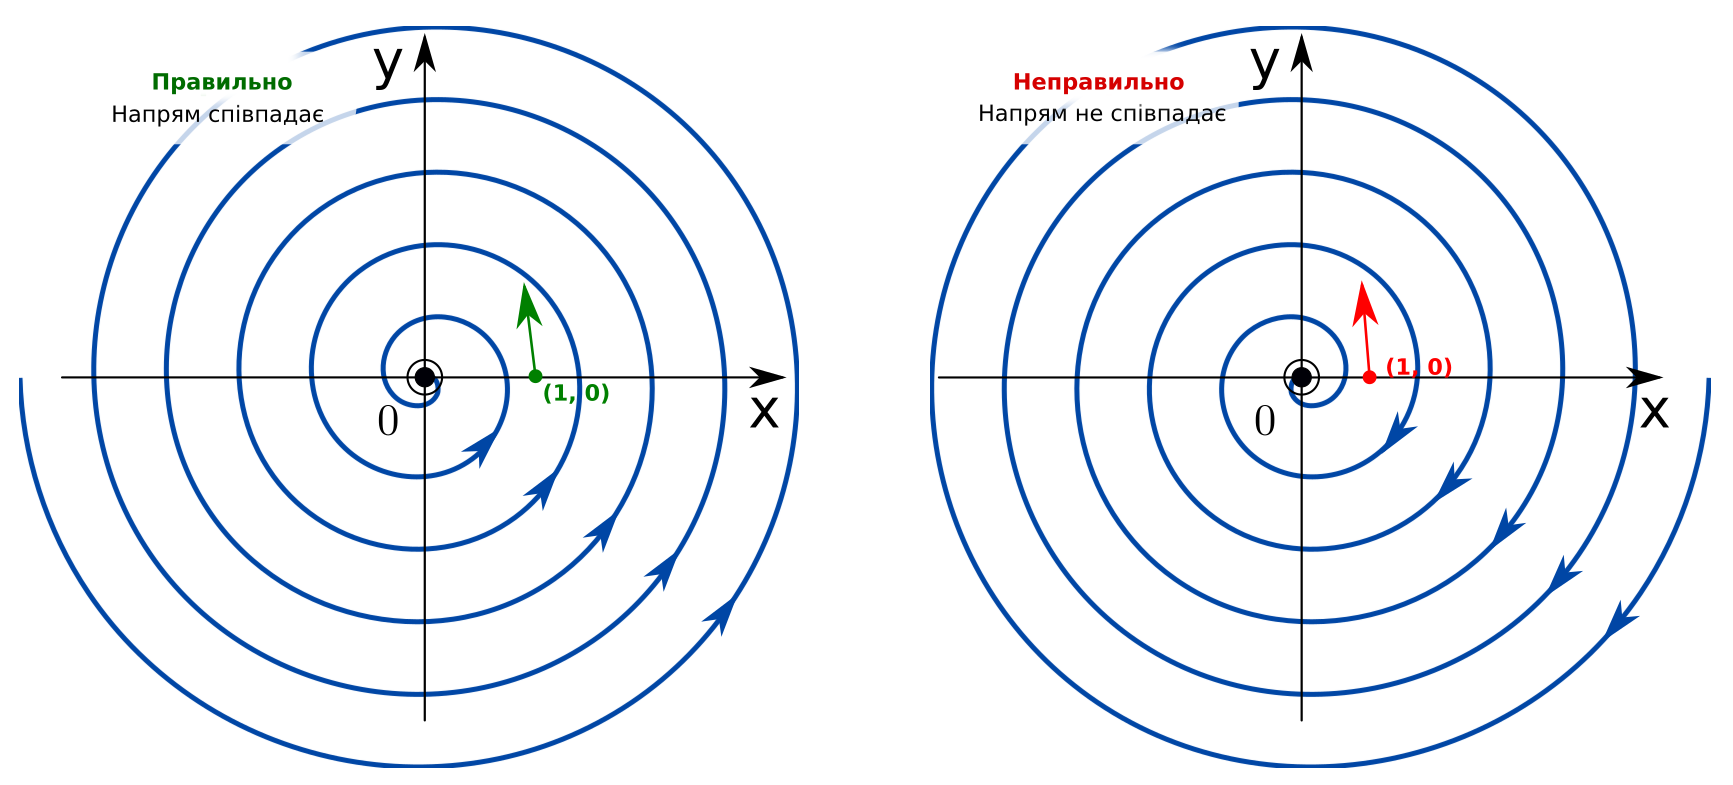
\includegraphics[scale=0.27]{assets/lectures_recent-b90426e3.png} \end{center}
Візьмемо точку (1, 0) для перевірки:

$$
\begin{bmatrix}
 \dot{x}\\
 \dot{y}
\end{bmatrix}\Bigg|_{(1,0)} - \begin{bmatrix}
 1 \\
 4
\end{bmatrix} \qquad \begin{gathered}
 x_k -1 = 1 \\
 y_k - 0 = 4
\end{gathered} \Rightarrow \begin{gathered}
 x_k = 2 \\
 y_k  = 4
\end{gathered}
$$
Отримали: $(1,0) \to (2, 4)$. Перевіримо за виглядом фазового портрета вище.
\end{example}

5.$ \lambda_{1,2} = \pm i \beta$. За таких власних чисел, фазовий портрет називається \textbf{центр.} (стійкий, але не асимптотично стійкий)
\begin{center} 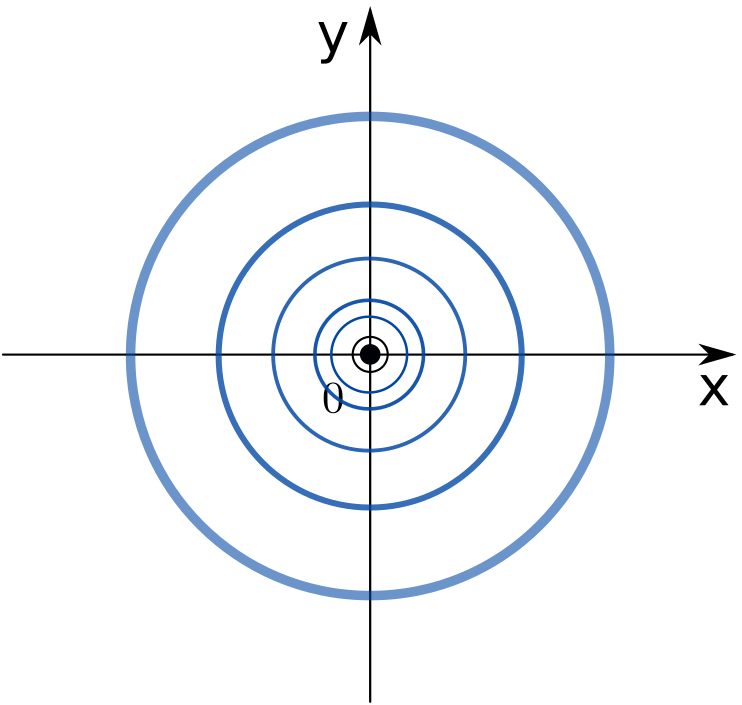
\includegraphics[scale=0.3]{assets/lectures_recent-2982f611.png} \end{center}

\begin{example}
    $$
    \begin{cases}
        \dot{x} = -2 x - 5y \\
        \dot{y} = 2x + 2y
    \end{cases} \qquad A = \begin{bmatrix}
     -2 & -5\\
     2 & 2
    \end{bmatrix}
    $$
    $$
    \det{(A - \lambda I)} = \begin{vmatrix}
      -2-\lambda & -5 \\
      2 & 2 -\lambda
    \end{vmatrix}  = \lambda^2 + 6 = 0 \Rightarrow \lambda = \pm i \sqrt{6} \Rightarrow \text{центр}
    $$
    Візьмемо т. (1, 0):
    $$
\begin{gathered}
\begin{bmatrix}
 \dot{x}\\
 \dot{y}
\end{bmatrix}\Bigg|_{(1,0)} = \begin{bmatrix}
 -2 \\
 2
\end{bmatrix} \\ \begin{cases}
  x_k -1 = -2\\
  y_k  - 0 = 2
\end{cases} \\
\begin{cases}
x_k = -1\\
    y_k  =2
\end{cases}
\end{gathered}\qquad    \begin{gathered} 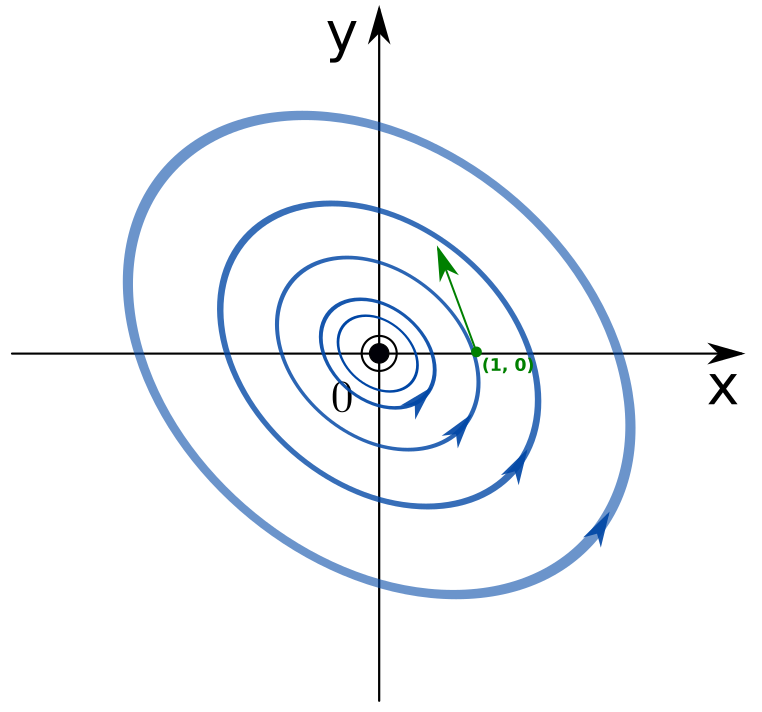
\includegraphics[scale=0.3]{assets/lectures_recent-1467e19e.png} \end{gathered}
    $$


\end{example}
6. Нехай $ \det A = 0$ (вирджений випадок).\\
$$
\det A  =  \begin{vmatrix}
  a & b\\
  c & d
\end{vmatrix} = ad - bc  = 0 \Rightarrow \frac{a}{c} = \frac{b}{d} = 0 \quad \begin{gathered}
 a = kc\\
 b = kd
\end{gathered}
$$
$$
\begin{cases}
    \dot{x} = ax+ by\\
    \dot{y} = k(ax + by)
\end{cases} \Rightarrow ax + by  = 0 \text{ - пряма положень рівноваги.}
$$

$$
\det ( A - \lambda I) = \begin{vmatrix}
  a - \lambda & b\\
  ka & kb - \lambda
\end{vmatrix} = (a-\lambda)*(kb- \lambda) - kab =
$$
$$
 = akb - a \lambda - kb \lambda +  \lambda^2 - kab = \lambda^2 - (a + kb) \lambda =0
 $$
 $$
 \lambda = 0 \qquad \lambda = a + bk
 $$

 a) Прямі паралельні власному вектору, що відповідає власному числу $\lambda =  a + bk$\\
 $\lambda > 0 $ - стрілки від нуля.\\
 $\lambda < 0 $ - стрілки до нуля.\\

 \begin{center} 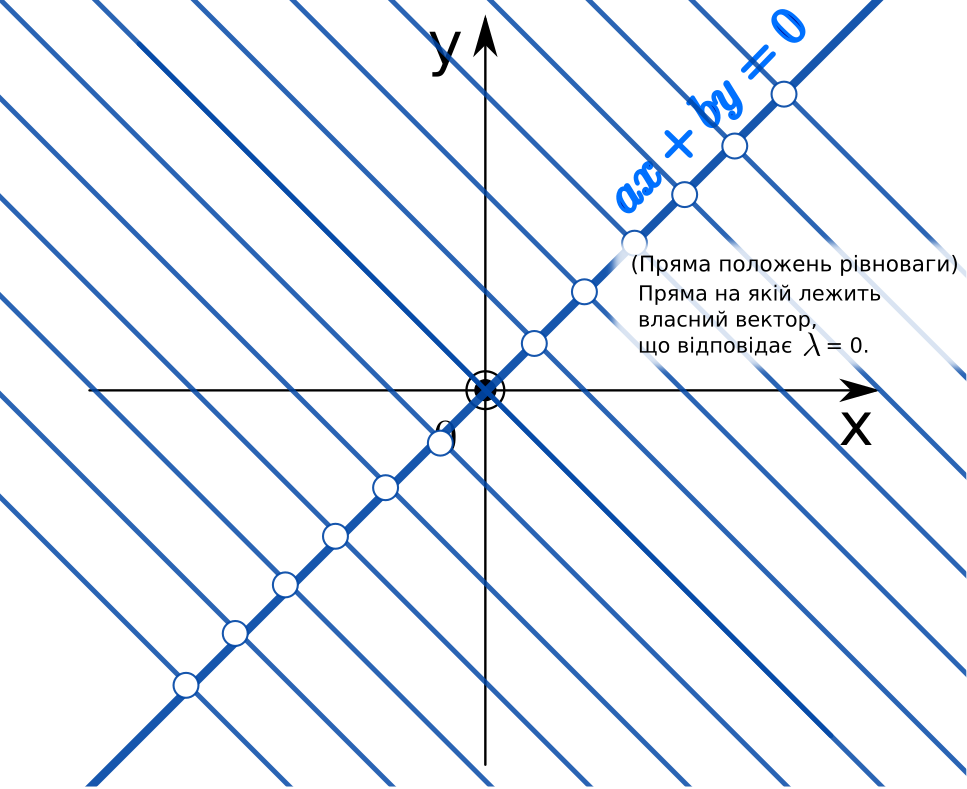
\includegraphics[scale=0.3]{assets/lectures_recent-058ceaff.png} \end{center}
b) $ \lambda_1 =  \lambda_2 = 0 \quad (a = - bk)$

\begin{center} 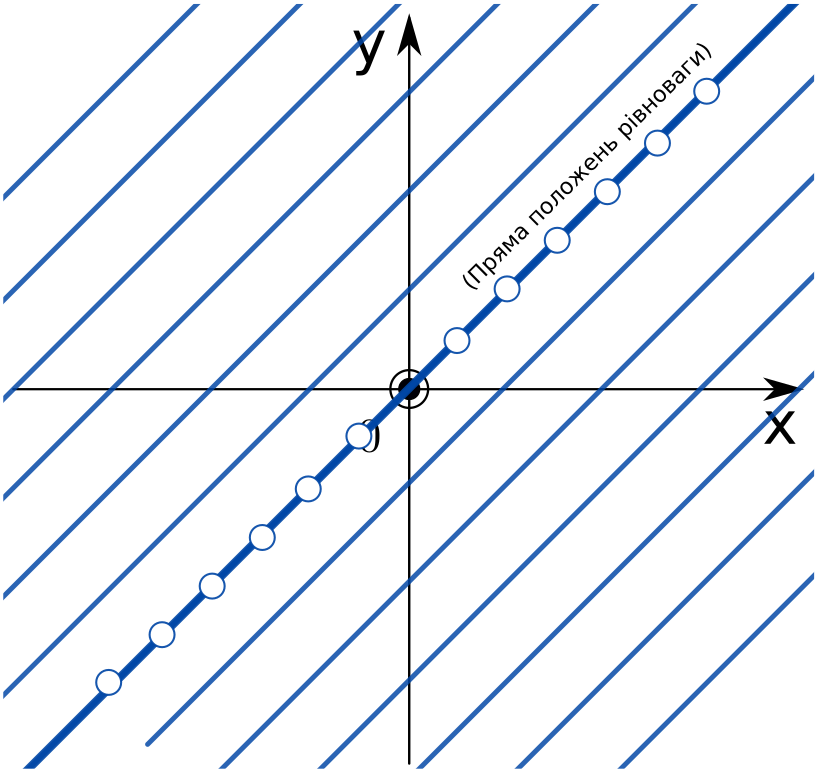
\includegraphics[scale=0.3]{assets/lectures_recent-49093f01.png} \end{center}

\end{document}
